\documentclass[letterpaper,11pt]{scrartcl}

\usepackage[T1]{fontenc}
\usepackage[utf8]{inputenc}
\usepackage{lmodern}
\usepackage{amsfonts,amsmath,amssymb,amsthm,mathtools}
\usepackage[letterpaper,margin=1.0in]{geometry}
\usepackage[english]{babel}
\setlength\parindent{1pt}
\setlength{\parskip}{0.75em}

% Universal v2 author package set (CI-safe by default)
\usepackage{wrapfig}
\usepackage{mdframed}
\usepackage[authoryear,round]{natbib}
\usepackage{bm}
\usepackage{multirow}
\usepackage{array}
\usepackage{verbatim}
\usepackage[normalem]{ulem}
\usepackage{thmtools}
\usepackage{setspace}
\usepackage{adjustbox}
\usepackage{graphicx}
\usepackage{subfig}
\usepackage[useregional]{datetime2}
\usepackage{enumitem}
\usepackage[most]{tcolorbox}
\tcbuselibrary{theorems}
\usepackage{longtable}
\usepackage{ltablex}
\usepackage{nccmath}
\usepackage{pifont}
\usepackage{sansmath}
\usepackage{booktabs,tabularx}
\usepackage{makecell}
\usepackage[ruled,vlined,linesnumbered]{algorithm2e}
\usepackage[dvipsnames]{xcolor}
\usepackage[colorlinks=true, citecolor=NavyBlue, linkcolor=RoyalBlue]{hyperref}

% Optional extended TikZ profile (opt-in)
% \usepackage{tikz}
% \usetikzlibrary{positioning,shadows,arrows,shapes,shapes.arrows,arrows.meta,trees,shapes.misc,shapes.geometric,decorations.pathreplacing,calc}

% Status symbols
\newcommand{\cmark}{\ding{51}}
\newcommand{\pmark}{\ding{108}}
\newcommand{\xmark}{\ding{55}}

% Generic colors
\definecolor{betterred}{RGB}{228,26,28}
\definecolor{betterblue}{RGB}{55,126,184}
\definecolor{afblue}{RGB}{0,0,102}

% Generic indicator
\newcommand{\Ind}{\boldsymbol{1}}

% Theorem environments
\newtheorem{definition}{Definition}
\newtheorem{theorem}{Theorem}
\newtheorem{assumption}{Assumption}
\newtheorem{example}{Example}
\newtheorem{lemma}{Lemma}
\newtheorem{conjecture}{Conjecture}
\newtheorem{proposition}{Proposition}
\newtheorem{corollary}{Corollary}
\newtheorem{remark}{Remark}

\tcolorboxenvironment{definition}{colback=gray!5!white,colframe=black,fonttitle=\bfseries,boxrule=0.5pt,breakable}
\tcolorboxenvironment{theorem}{colback=gray!5!white,colframe=black,fonttitle=\bfseries,boxrule=0.5pt,breakable}
\tcolorboxenvironment{corollary}{colback=gray!5!white,colframe=black,fonttitle=\bfseries,boxrule=0.5pt,breakable}
\tcolorboxenvironment{lemma}{colback=gray!5!white,colframe=black,fonttitle=\bfseries,boxrule=0.5pt,breakable}
\tcolorboxenvironment{proposition}{colback=gray!5!white,colframe=black,fonttitle=\bfseries,boxrule=0.5pt,breakable}
\tcolorboxenvironment{remark}{colback=gray!5!white,colframe=black,fonttitle=\bfseries,boxrule=0.5pt,breakable}
\tcolorboxenvironment{assumption}{colback=white,colframe=black,fonttitle=\bfseries,boxrule=0.5pt,breakable}


\title{\textbf{Prediction-Powered Data Fusion for Treatment Effect Estimation}}
\author{Yonghan Jung}
\date{Working draft, \today}

\begin{document}
\maketitle
\allowdisplaybreaks

\begin{abstract}
Randomized controlled trials identify causal effects under transparent design assumptions, but their sample sizes can make average and conditional treatment-effect estimation imprecise. Observational studies are often larger and can yield accurate outcome predictions, but those predictions need not be causal. We develop a model-agnostic prediction-powered framework that keeps the randomized trial as the causal anchor while using observational outcome models and covariates through two tunable channels. The coefficient \(\lambda\) changes the outcome regression inside an RCT-valid pseudo-outcome, and \(\omega\) introduces a prediction-powered control variate centered across the two samples.

For the average treatment effect, we derive exact conditional unbiasedness, an exact two-sample variance formula, the joint population variance minimizer, its population-orthogonal simplification, and an honest plug-in algorithm. For conditional effects, we formulate a prediction-powered squared-loss learner from an RCT-valid AIPW pseudo-outcome, distinguish target preservation from empirical loss-variance tuning, and give implementable linear-sieve and frozen-neural-basis versions. We outline an R-loss analogue only as a prospective extension requiring a separate derivation. Exact density-ratio transport covers unequal covariate marginals, while loss-targeted balancing gives an approximate alternative with explicit drift. Existing simulations support the ATE construction in several small-trial regimes. CATE experiments and real-outcome analyses remain planned, so the present empirical evidence does not establish a universal finite-sample improvement guarantee.

\end{abstract}

\tableofcontents
\newpage

\begingroup
\allowdisplaybreaks
\sloppy
\section{Introduction}
\label{sec:introduction}
\subsection{Categorized literature review}
\label{sec:literature}

\textbf{Prediction-powered inference.} Prediction-powered inference uses a large set of machine predictions together with a smaller labeled sample, correcting the prediction-based estimate with labeled residuals so that the statistical target does not require the predictor to be correct \citep{angelopoulos2023ppi}. This separation between predictive quality and inferential validity is the starting point for the present construction. Randomized observations play the role of causally valid labeled data, while observational outcome models supply potentially useful predictions.

\textbf{Adaptive prediction-powered inference.} PPI++ introduces data-adaptive power tuning that adjusts how strongly predictions enter an estimating equation and reports computational and statistical gains over the original construction \citep{angelopoulos2024ppipp}. Its central lesson is that a prediction should be used in proportion to its empirical value rather than being accepted as truth. Our coefficient $\omega$ follows this control-variate logic, but the target and score are causal quantities identified by the randomized design.

\textbf{Causal data fusion and transport.} General causal data-fusion theory distinguishes data collected under different regimes and populations and asks whether a target causal query is identified from their combination \citep{bareinboim2016fusion}. Reviews of causal data integration likewise separate randomized trials, observational studies, historical controls, and heterogeneous target populations \citep{shi2022integration}. The present paper assumes that the trial already identifies the target effect and studies an estimation question: how can observational predictions improve precision without replacing randomized identifying information?

\textbf{Combining randomized and observational estimates.} Existing estimators combine experimental and observational effect estimates through shrinkage, bias detection, or adaptive weighting. Shrinkage estimators can reduce risk when observational bias is sufficiently controlled \citep{rosenman2020shrinkage}, while adaptive combination methods move toward the randomized estimator when observational bias is detected \citep{cheng2021adaptive}. These approaches combine effect estimates from the two sources. Our construction instead inserts the observational outcome model into an RCT-valid pseudo-outcome and separately centers a prediction-based covariate statistic.

\textbf{CATE learners and orthogonal losses.} Meta-learners convert standard regression algorithms into conditional effect estimators \citep{kunzel2019metalearners}. The R-learner residualizes outcomes and treatments to isolate treatment-effect heterogeneity \citep{nie2020rlearner}, while doubly robust pseudo-outcome regression can retain favorable error structure under nuisance estimation \citep{kennedy2022drlearner}. Direct multi-source learners have also been proposed for heterogeneous causal data fusion \citep{li2022directfusion}. These results motivate treating the prediction-powered construction as a loss wrapper that can be paired with a linear sieve or a fixed learned representation.

\textbf{Covariate shift and balancing.} When trial and observational covariate marginals differ, exact density-ratio weighting transports fixed covariate functions between populations. Riesz-representer methods provide an optimization perspective on such linear functionals and on debiasing \citep{chernozhukov2021riesz}. Density-ratio estimation, generic balancing, and Riesz learning are established tools. The project-specific question is whether they can be targeted to the generated CATE loss class $\{(\widehat g-t)^2:t\in\mathcal T\}$, where $\widehat g$ is the fitted OBS treatment-effect prediction defined later in Equation~\eqref{eq:obs-effect-prediction}, while preserving an RCT-defined risk; we treat this specialization as a working research direction rather than a settled novelty claim.

\section{Background and Problem Setting}
\label{sec:setup}

\subsection{Prediction-powered inference and PPI++}
\label{sec:ppi-background}

Let \((X_i,Y_i)\), \(i=1,\ldots,n\), be labeled pairs and let \(\widetilde X_j\), \(j=1,\ldots,N\), be unlabeled covariates. Suppose a fixed predictor supplies \(f(X_i)\) and \(f(\widetilde X_j)\). For a mean target, the elementary prediction-powered decomposition is
\begin{align}
\widehat\mu_{\mathrm{PPI}}
&=
\frac1N\sum_{j=1}^N f(\widetilde X_j)
+
\frac1n\sum_{i=1}^n\{Y_i-f(X_i)\}.
\end{align}
When labeled and unlabeled covariates share a marginal law and the two samples are independent, the prediction term and residual correction sum to the labeled-population mean for every fixed predictor \(f\). PPI++ generalizes this idea by tuning the strength of the prediction contribution. In our construction, \(\omega\) is the PPI-style scale on a mean-zero prediction control variate. By contrast, \(\lambda\) blends trial and observational outcome regressions inside an RCT-valid score; it is not the scale on the external prediction mean.

\subsection{RCT--OBS problem setting and notation}
\label{sec:rct-obs-setting}

We observe independent samples
\begin{align}
D_R
&=\{V_i^R=(X_i^R,A_i^R,Y_i^R):i=1,\ldots,n\}\sim P_R^{\otimes n},
\\
D_O
&=\{V_j^O=(X_j^O,A_j^O,Y_j^O):j=1,\ldots,N\}\sim P_O^{\otimes N},
\end{align}
where \(X\) is a covariate vector, \(A\in\{0,1\}\) is treatment, and \(Y\) is the observed outcome. For a function \(h\), write \(\mathbb P_{R,n}h=n^{-1}\sum_i h(V_i^R)\) and \(\mathbb P_{O,N}h=N^{-1}\sum_j h(V_j^O)\).

For the exact adaptive results, these displayed samples are the final-evaluation blocks. Separate RCT and OBS blocks \(D_R^{\mathrm{tr}},D_O^{\mathrm{tr}}\) train nuisance and ratio functions, and separate blocks \(D_R^{\mathrm{tu}},D_O^{\mathrm{tu}}\) select coefficients. Define the pre-evaluation sigma-field
\begin{align}
\mathcal F
&=
\sigma\!\left(
D_R^{\mathrm{tr}},D_O^{\mathrm{tr}},
D_R^{\mathrm{tu}},D_O^{\mathrm{tu}},
\text{prespecified split randomness}
\right).
\label{eq:pre-evaluation-field}
\end{align}
The split assignments are fixed in advance or independently randomized, with their randomness included in \(\mathcal F\). Conditional on \(\mathcal F\), every fitted nuisance, ratio, basis, and selected coefficient is fixed and
\begin{align}
\mathcal L(D_R,D_O\mid\mathcal F)
&=
P_R^{\otimes n}\otimes P_O^{\otimes N}.
\label{eq:evaluation-product-law}
\end{align}
For fixed-coefficient statements the tuning blocks may be empty.

Let \(Y(1)\) and \(Y(0)\) denote potential outcomes. The RCT-population conditional and average treatment effects are
\begin{align}
\tau(x)
&=\mathbb E_R\{Y(1)-Y(0)\mid X=x\},
&
\theta
&=\mathbb E_R\{\tau(X)\}.
\end{align}

\begin{assumption}[Trial identification]
\label{ass:trial}
Consistency holds, \(\{Y(0),Y(1)\}\perp A\mid X\) under \(P_R\), and the known trial propensity \(e(x)=P_R(A=1\mid X=x)\) satisfies \(\epsilon<e(X)<1-\epsilon\) almost surely for a constant \(\epsilon>0\).
\end{assumption}

\begin{assumption}[Common covariate marginal]
\label{ass:common-marginal}
\label{ass:covariate}
The trial and observational covariates have the same marginal law, \(P_R^X=P_O^X\). This assumption does not equate the treatment or outcome mechanisms across sources, and the observational treatment contrast may remain confounded.
\end{assumption}

\begin{assumption}[Exact covariate transport]
\label{ass:exact-transport}
Under covariate shift, \(P_R^X\ll P_O^X\) and the exact density ratio
\begin{align}
r(x)
&=\frac{dP_R^X}{dP_O^X}(x),
&
\mathbb E_O\{r(X)h(X)\}
&=\mathbb E_R\{h(X)\}
\end{align}
is available for every required integrable function \(h\). The common-marginal model is the special case \(r=1\).
\end{assumption}

\begin{assumption}[Honest evaluation and moments]
\label{ass:honest-evaluation}
Every fitted object used in an exact identity is \(\mathcal F\)-measurable, the final observations satisfy Equation~\eqref{eq:evaluation-product-law}, and every displayed conditional moment is finite almost surely. Square-integrability and stronger moment conditions are stated locally when variance estimation or Wald inference requires them.
\end{assumption}

The exact-r results use Assumption~\ref{ass:exact-transport}; their common-marginal corollaries use Assumption~\ref{ass:common-marginal} and set \(r=1\). Neither version assumes that the OBS treatment contrast is causal.

Let \(\widehat\mu_R=(\widehat\mu_{R,0},\widehat\mu_{R,1})\) and \(\widehat\mu_O=(\widehat\mu_{O,0},\widehat\mu_{O,1})\) be outcome regressions fitted on the two sources. Define
\begin{align}
g(x)
&=\widehat\mu_{O,1}(x)-\widehat\mu_{O,0}(x),
\\
\varphi(V;q)
&=q_1(X)-q_0(X)
+\frac{A}{e(X)}\{Y-q_1(X)\}
-\frac{1-A}{1-e(X)}\{Y-q_0(X)\}.
\end{align}
\begin{proposition}[RCT-validity for an arbitrary outcome regression]
\label{prop:pseudo-validity-active}
\label{prop:pseudo-validity}
Under Assumptions~\ref{ass:trial} and \ref{ass:honest-evaluation}, every fixed \(q\) with finite first moments satisfies
\begin{align}
\mathbb E_R\{\varphi(V;q)\mid X\}
&=\tau(X).
\label{eq:pseudo-valid}
\end{align}
\end{proposition}
For \(\lambda\in\mathbb R\), set
\begin{align}
\widehat\mu_\lambda
&=(1-\lambda)\widehat\mu_R+\lambda\widehat\mu_O,
&
Z_\lambda
&=\varphi(V;\widehat\mu_\lambda)
=Z_0+\lambda\Delta,
&
\Delta
&=Z_1-Z_0.
\end{align}
Equation~\eqref{eq:pseudo-valid} implies \(\mathbb E_R(Z_\lambda\mid X)=\tau(X)\) and \(\mathbb E_R(\Delta\mid X)=0\). The observational contrast \(g\) is used only as a prediction and need not equal \(\tau\).

\subsection{Existing data-fusion estimators}
\label{sec:existing-fusion}

Three existing strategies provide the nearest comparisons. First, shrinkage methods combine an unbiased experimental estimate with a potentially biased observational estimate and trade variance against observational bias \citep{rosenman2020shrinkage}. Second, adaptive RCT--OBS estimators estimate source-specific conditional effects and downweight the observational estimator when its discrepancy from the trial is large \citep{cheng2021adaptive}. Third, direct multi-source learners construct weighted pseudo-outcomes for heterogeneous effects across sources \citep{li2022directfusion}. Our estimator differs at the level of the fusion object: \(\lambda\) changes the nuisance regression inside a trial-valid score, while \(\omega\) centers a fixed prediction across study covariate samples. Neither channel treats the observational treatment contrast as identified causal truth.

Within the adaptive and integrative line, the elastic procedure of \citet{yang2023elastic} tests whether real-world data are sufficiently compatible with the randomized trial before pooling information for prespecified effect modifiers. The confounding-function approach of \citet{yang2025confounding} instead introduces and jointly estimates an HTE function and an observational confounding function under explicit cross-source identification conditions. These methods use observational outcomes through a poolability decision or an identified confounding-function model; our two fusion channels retain the RCT-valid score as the causal anchor.

\section{Prediction-Powered Fusion for the ATE}
\label{sec:ate}

\subsection{Estimator and exact variance}

For fixed \((\lambda,\omega)\), define
\begin{align}
\widehat\theta_r(\lambda,\omega)
&=
\mathbb P_{R,n}Z_\lambda
+
\omega\left\{
\mathbb P_{O,N}\{r(X)g(X)\}
-
\mathbb P_{R,n}g(X)
\right\}.
\label{eq:ate-estimator}
\end{align}
Here \(Z_\lambda\) is the fusion score in
Definition~\ref{def:fusion-score}, \(g\) is defined in
Equation~\eqref{eq:obs-effect-prediction}, and \(r\) is the transport ratio in
Assumption~\ref{ass:exact-transport}. At the coefficient origin,
\begin{align*}
\widehat\theta_r(0,0)
&=\mathbb P_{R,n}Z_0
=\widehat\theta_{\mathrm{AIPW},R},
\end{align*}
so the proposed family contains the RCT-only AIPW estimator from
Definition~\ref{def:rct-only-aipw} exactly.
The first term averages an RCT-valid pseudo-outcome. Under Assumption~\ref{ass:exact-transport}, the expression in braces is a mean-zero control variate; under Assumption~\ref{ass:common-marginal}, this is the special case \(r=1\). Thus, the RCT identifies the target, \(\lambda\) changes within-covariate score noise, and \(\omega\) uses the large OBS covariate sample to remove predictable between-covariate variation.

\begin{theorem}[Exact mean and variance under honest evaluation]
\label{thm:ate-variance}
\label{thm:ate-exact-r}
Under Assumptions~\ref{ass:trial}, \ref{ass:exact-transport}, and
\ref{ass:honest-separation}, suppose \(n,N>0\) and the displayed scores are
square-integrable. Every fixed \((\lambda,\omega)\) then satisfies
\begin{align}
\mathbb E\{\widehat\theta_r(\lambda,\omega)\}
&=\theta,
\\
\operatorname{Var}\{\widehat\theta_r(\lambda,\omega)\}
&=
\frac1n\operatorname{Var}_R\{Z_\lambda-\omega g(X)\}
+
\frac{\omega^2}{N}\operatorname{Var}_O\{r(X)g(X)\}.
\label{eq:ate-variance}
\end{align}
Equivalently, the law of total variance gives the within-/between-covariate decomposition
\begin{align}
\operatorname{Var}\{\widehat\theta_r(\lambda,\omega)\}
&=
\frac1n\mathbb E_R\{\operatorname{Var}_R(Z_\lambda\mid X)\}
+\frac1n\operatorname{Var}_R\{\tau(X)-\omega g(X)\}
+\frac{\omega^2}{N}\operatorname{Var}_O\{r(X)g(X)\}.
\label{eq:ate-within-between}
\end{align}
\end{theorem}

The mean follows from \(\mathbb E_R(Z_\lambda)=\theta\) and \(\mathbb E_O(rg)=\mathbb E_R(g)\). The variance follows after rewriting Equation~\eqref{eq:ate-estimator} as the sum of independent RCT and OBS empirical means.

\begin{corollary}[Common-marginal specialization]
\label{cor:ate-common-active}
Under Assumptions~\ref{ass:trial}, \ref{ass:common-marginal}, and
\ref{ass:honest-separation}, set \(r=1\) in
Theorem~\ref{thm:ate-variance}. Then Equation~\eqref{eq:ate-estimator} is
exactly unbiased, and its OBS variance term is
\(\omega^2\operatorname{Var}_R\{g(X)\}/N\).
\end{corollary}

\subsection{Joint and population-orthogonal oracles}

Throughout this subsection, Assumption~\ref{ass:honest-separation} remains in
force, \(n\) and \(N\) are positive, and the displayed random variables have
finite second moments.

\begin{definition}[ATE variance-quadratic objects]
\label{def:ate-variance-objects}
Define the five population moments
\begin{align}
A&\triangleq\operatorname{Var}_R(\Delta),
&
B&\triangleq\operatorname{Var}_R(g)+\frac nN\operatorname{Var}_O(rg),
\\
C&\triangleq\operatorname{Cov}_R(Z_0,\Delta),
&
D&\triangleq\operatorname{Cov}_R(Z_0,g),
&
E&\triangleq\operatorname{Cov}_R(\Delta,g).
\label{eq:ate-moments}
\end{align}
The moment \(A\) is the curvature cost of changing the outcome-regression blend
\(\lambda\). The moment \(B\) is the curvature cost of the prediction-powered
scale \(\omega\), including both the RCT subtraction and the scaled OBS
addition. The moment \(C\) is the baseline-score covariance that determines the
linear slope in the \(\lambda\) direction. The moment \(D\) is the
baseline-prediction covariance that determines the linear slope in the
\(\omega\) direction, with a minus sign because the RCT score contains
\(-\omega g\). The moment \(E\) is the interaction covariance coupling the two
coefficients through the cross-term \(-2E\lambda\omega\).

Collect these moments and coefficients as
\begin{align}
\mathbf H_{\mathrm{ATE}}
&\triangleq
\begin{pmatrix}A&-E\\-E&B\end{pmatrix},
&
\boldsymbol\ell
&\triangleq
\begin{pmatrix}C\\-D\end{pmatrix},
&
\beta
&\triangleq
\begin{pmatrix}\lambda\\\omega\end{pmatrix},
\end{align}
\end{definition}

\begin{proposition}[ATE variance quadratic and positive-semidefinite curvature]
\label{prop:ate-variance-quadratic}
Under the standing conditions of this subsection, the compact variance in
Equation~\eqref{eq:ate-variance} is
\begin{align}
\operatorname{Var}\{\widehat\theta_r(\beta)\}
&=
\frac1n\left\{
\operatorname{Var}_R(Z_0)+2\boldsymbol\ell^\top\beta+\beta^\top\mathbf H_{\mathrm{ATE}}\beta
\right\}.
\label{eq:ate-quadratic}
\end{align}
Moreover, \(\mathbf H_{\mathrm{ATE}}\) is positive semidefinite because, for
every \((u,v)\in\mathbb R^2\),
\begin{align}
\begin{pmatrix}u&v\end{pmatrix}
\mathbf H_{\mathrm{ATE}}
\begin{pmatrix}u\\v\end{pmatrix}
&=
\operatorname{Var}_R(u\Delta-vg)
+\frac nN v^2\operatorname{Var}_O(rg)
\geq0.
\end{align}
\end{proposition}

The variance in Equation~\eqref{eq:ate-quadratic} contains the RCT-only
baseline \(\operatorname{Var}_R(Z_0)/n\), which no coefficient can change.
Coefficient selection can therefore focus on the remaining quadratic. Its
positive-semidefinite curvature guarantees that this reduced objective cannot
decrease without bound.

\begin{definition}[ATE coefficient objective]
\label{def:ate-coefficient-objective}
Define the coefficient-dependent part of the scaled variance by
\begin{align*}
\mathcal J_{\mathrm{ATE}}(\beta)
&\triangleq
2\boldsymbol\ell^\top\beta
+\beta^\top\mathbf H_{\mathrm{ATE}}\beta.
\end{align*}
\end{definition}

\begin{proposition}[Population orthogonality of the fusion directions]
\label{prop:ate-population-orthogonality}
Under Assumptions~\ref{ass:trial} and \ref{ass:honest-separation}, the two
endpoint scores have the same conditional target:
\begin{align*}
\mathbb E_R(Z_a\mid X)
&=\tau(X),
\qquad a\in\{0,1\},
\\
\mathbb E_R(\Delta\mid X)
&=0.
\end{align*}
Because \(g\) is a fixed function of \(X\), it follows that
\begin{align}
E
&=\operatorname{Cov}_R\{\Delta,g(X)\}=0,
&
D
&=\operatorname{Cov}_R\{\tau(X),g(X)\}.
\label{eq:ate-population-orthogonality}
\end{align}
\end{proposition}

This result formalizes the purpose of the outcome-regression blend: changing
\(\lambda\) changes pseudo-outcome noise without changing its conditional CATE
target. The zero population interaction separates the two oracle directions.
We nevertheless retain the general \(E\) term because its tuning-sample
analogue \(\widehat E\) is generally nonzero, and the empirical joint quadratic
program must account for that sampling fluctuation.

\begin{proposition}[Equivalent ATE oracle objectives]
\label{prop:ate-argmin-equivalence}
For every nonempty feasible set \(\mathcal B\subseteq\mathbb R^2\), the two
argmin sets, possibly empty when the infimum is not attained, satisfy
\begin{align*}
\operatorname*{arg\,min}_{\beta\in\mathcal B}
\operatorname{Var}\{\widehat\theta_r(\beta)\}
&=
\operatorname*{arg\,min}_{\beta\in\mathcal B}
\mathcal J_{\mathrm{ATE}}(\beta).
\end{align*}
\end{proposition}

Positive semidefiniteness means that the variance objective cannot curve
downward along any direction \((u,v)\). For this two-dimensional matrix, the
stronger condition \(AB-E^2>0\), together with positive semidefiniteness, makes
\(\mathbf H_{\mathrm{ATE}}\) positive definite and invertible. It turns a
possibly flat quadratic into one with a unique unrestricted minimizer.

\begin{definition}[Joint and ridge population oracles]
\label{def:ate-joint-ridge-oracles}
When \(AB-E^2>0\), define the unrestricted joint oracle by
\begin{align*}
\beta_{\mathrm{joint}}^\star
&\triangleq
\operatorname*{arg\,min}_{\beta\in\mathbb R^2}
\operatorname{Var}\{\widehat\theta_r(\beta)\}
=
\operatorname*{arg\,min}_{\beta\in\mathbb R^2}
\mathcal J_{\mathrm{ATE}}(\beta).
\end{align*}
The equality of the two argmin sets follows from
Proposition~\ref{prop:ate-argmin-equivalence}.
For a prespecified \(\rho>0\), define the ridge-stabilized population oracle by
\begin{align*}
\beta_\rho^\star
&\triangleq
\operatorname*{arg\,min}_{\beta\in\mathbb R^2}
\left\{\mathcal J_{\mathrm{ATE}}(\beta)+\rho\lVert\beta\rVert_2^2\right\}.
\end{align*}
Let \(I_2\) denote the \(2\times2\) identity matrix.
\end{definition}

\begin{theorem}[Joint and ridge population oracles]
\label{thm:joint-oracle}
If \(AB-E^2>0\), the joint oracle in
Definition~\ref{def:ate-joint-ridge-oracles} is unique and
\begin{align}
\beta_{\mathrm{joint}}^\star
&=
\begin{pmatrix}
\lambda_{\mathrm{joint}}^\star\\
\omega_{\mathrm{joint}}^\star
\end{pmatrix}
=-\mathbf H_{\mathrm{ATE}}^{-1}\boldsymbol\ell
=
\begin{pmatrix}
(ED-BC)/(AB-E^2)\\
(AD-EC)/(AB-E^2)
\end{pmatrix}.
\label{eq:joint-oracle}
\end{align}
For every \(\rho>0\), whether or not \(\mathbf H_{\mathrm{ATE}}\) is singular,
the ridge oracle is unique and
\begin{align}
\beta_\rho^\star
&=-(\mathbf H_{\mathrm{ATE}}+\rho I_2)^{-1}\boldsymbol\ell.
\label{eq:ridge-oracle}
\end{align}
\end{theorem}

Theorem~\ref{thm:joint-oracle} locates the joint minimum of the two-coefficient variance quadratic. Corollary~\ref{cor:joint-oracle-variance} answers the distinct comparison question: it evaluates the quadratic at that minimum and quantifies the improvement relative to the RCT-only origin \(\beta=0\). The general interaction \(E\) is retained here because its empirical analogue \(\widehat E\) need not vanish, even though the exact population model later implies \(E=0\).

\begin{remark}[Singular or constrained curvature]
If \(\mathbf H_{\mathrm{ATE}}\) is singular, an unpenalized joint minimum can
lie along a flat set rather than at a unique point. The Moore--Penrose and
null-space characterization, as well as existence and uniqueness results under
coefficient constraints, are recorded in Appendix~\ref{app:proofs}. The ridge
oracle remains unique for every \(\rho>0\). In implementation we minimize the
continuous quadratic over a prespecified compact box, which guarantees at least
one constrained solution.
\end{remark}

\begin{corollary}[Joint-oracle variance reduction]
\label{cor:joint-oracle-variance}
Let \(\sigma_0^2=\operatorname{Var}_R(Z_0)\) and \(\mathcal V_0=\sigma_0^2/n\) be the variance at \((\lambda,\omega)=(0,0)\). If \(AB-E^2>0\), the unrestricted joint oracle has
\begin{align*}
V_{\min}
&=
\mathcal V_0-
\frac1n
\frac{BC^2-2ECD+AD^2}{AB-E^2},
\\
\mathcal V_0-V_{\min}
&=
\frac1n\boldsymbol\ell^\top\mathbf H_{\mathrm{ATE}}^{-1}\boldsymbol\ell.
\end{align*}
The reduction is nonnegative and is strictly positive exactly when \(\boldsymbol\ell\neq0\), equivalently when \((C,D)\neq(0,0)\). Under population orthogonality \(E=0\) and \(A,B>0\), this specializes to
\begin{align*}
V_{\min}
&=
\mathcal V_0-
\frac1n\left(\frac{C^2}{A}+\frac{D^2}{B}\right).
\end{align*}
\end{corollary}

By Proposition~\ref{prop:ate-population-orthogonality}, the interaction term
\(-2E\lambda\omega\) vanishes. When \(A,B>0\), the population oracle therefore
separates:
\begin{align}
\lambda^\star
&=-\frac CA,
&
\omega^\star
&=\frac DB.
\label{eq:axis-oracle}
\end{align}
If \(A=0\), conditional mean zero forces \(\Delta=0\) almost surely and the \(\lambda\) direction is flat. If \(B=0\), both \(g(X)\) and \(r(X)g(X)\) are constant on their relevant supports, so the prediction-powered correction is samplewise zero and the \(\omega\) direction is flat. Under the common covariate marginal,
\begin{align*}
B
&=\left(1+\frac nN\right)\operatorname{Var}_R\{g(X)\}.
\end{align*}
For the rectangular box \(\mathcal B_\beta\) and positive \(A,B\), population orthogonality gives the coordinatewise projection
\begin{align*}
\lambda_{\mathcal B_\beta}^\star
&=\Pi_{[L_\lambda,U_\lambda]}(-C/A),
&
\omega_{\mathcal B_\beta}^\star
&=\Pi_{[L_\omega,U_\omega]}(D/B).
\end{align*}
For a coupled constraint or a nonzero interaction, the original quadratic must be minimized directly. The population oracle weakly improves the variance objective whenever \((0,0)\) is feasible. Estimated coefficients have no universal finite-sample no-harm guarantee.

\subsection{Estimable honest algorithm}

For random quantities \(U\) and \(W\) evaluated on
\(D_S^{\mathrm{tune}}\), assume \(n_S^{\mathrm{tune}}\geq2\). Conditional on
the fixed nuisance fits, let
\(\widehat{\operatorname{Cov}}_{S,\mathrm{tune}}(U,W)\) denote their usual
Bessel-corrected sample covariance and define
\(\widehat{\operatorname{Var}}_{S,\mathrm{tune}}(U)
\triangleq\widehat{\operatorname{Cov}}_{S,\mathrm{tune}}(U,U)\). The factor
\(n/N\) below uses the evaluation-sample sizes whose variance is optimized.

Using the tuning samples, compute
\begin{align}
\widehat A&=\widehat{\operatorname{Var}}_{R,\mathrm{tune}}(\Delta),
&
\widehat B&=\widehat{\operatorname{Var}}_{R,\mathrm{tune}}(g)
+\frac nN\widehat{\operatorname{Var}}_{O,\mathrm{tune}}(rg),
\\
\widehat C&=\widehat{\operatorname{Cov}}_{R,\mathrm{tune}}(Z_0,\Delta),
&
\widehat D&=\widehat{\operatorname{Cov}}_{R,\mathrm{tune}}(Z_0,g),
&
\widehat E&=\widehat{\operatorname{Cov}}_{R,\mathrm{tune}}(\Delta,g).
\end{align}
Define
\begin{align*}
\widehat{\mathbf H}_{\mathrm{ATE}}
&=
\begin{pmatrix}
\widehat A&-\widehat E\\
-\widehat E&\widehat B
\end{pmatrix},
&
\widehat{\boldsymbol\ell}
&=
\begin{pmatrix}\widehat C\\-\widehat D\end{pmatrix},
&
\widehat d
&=
\widehat A\widehat B-\widehat E^2.
\end{align*}
Choose positive thresholds \(t_A,t_B,t_{\det}\) before observing the tuning outcomes. The population-orthogonality axis rule is
\begin{align*}
\widehat\lambda_{\mathrm{axis}}
&=
\begin{cases}
-\widehat C/\widehat A,&\widehat A>t_A,\\
0,&\widehat A\leq t_A,
\end{cases}
&
\widehat\omega_{\mathrm{axis}}
&=
\begin{cases}
\widehat D/\widehat B,&\widehat B>t_B,\\
0,&\widehat B\leq t_B.
\end{cases}
\end{align*}
When \(\widehat A>t_A\), \(\widehat B>t_B\), and \(\widehat d>t_{\det}\), the unrestricted empirical joint rule is
\begin{align*}
\widehat\lambda_{\mathrm{joint}}
&=
\frac{\widehat E\widehat D-\widehat B\widehat C}{\widehat d},
&
\widehat\omega_{\mathrm{joint}}
&=
\frac{\widehat A\widehat D-\widehat E\widehat C}{\widehat d}.
\end{align*}
For the prespecified nonempty compact box \(\mathcal B_\beta=[L_\lambda,U_\lambda]\times[L_\omega,U_\omega]\) containing the origin, the boundary-correct empirical choice is
\begin{align*}
\widehat\beta_{\mathcal B_\beta}
&\in
\operatorname*{arg\,min}_{\beta\in\mathcal B_\beta}
\left\{
2\widehat{\boldsymbol\ell}^\top\beta
+\beta^\top\widehat{\mathbf H}_{\mathrm{ATE}}\beta
\right\}.
\end{align*}
If the unrestricted joint rule lies outside \(\mathcal B_\beta\), this quadratic program must be solved rather than clipping its coordinates separately; rectangular coordinate-wise clipping is exact only after imposing \(\widehat E=0\). For the joint rule, if a required threshold fails or the quadratic solver is numerically unstable, the prespecified fallback is \((0,0)\); the axis rule uses its coordinate-specific threshold definitions above.

The population-orthogonality plug-in imposes \(\widehat E=0\) and uses \((-\widehat C/\widehat A,\widehat D/\widehat B)\). The empirical joint minimizer retains \(\widehat E\) and applies Equation~\eqref{eq:joint-oracle}. The two rules differ because sample orthogonality is not exact.

Each sample covariance is conditionally unbiased for its corresponding
fixed-score population moment given the nuisance fits, but the ratios defining
\(\widehat\lambda\) and \(\widehat\omega\) are nonlinear and are not generally
unbiased for the population oracle coefficients. The thresholds and feasible
box control instability; they do not turn these selected coefficients into
finite-sample oracle estimates.

The displayed analytic ratios apply only when their corresponding denominator thresholds pass. Imposing \(\widehat E=0\) does not assert that the realized tuning covariance vanishes. It applies the proven population restriction \(E=0\) before solving the sample problem. Retaining \(\widehat E=\widehat{\operatorname{Cov}}_{R,\mathrm{tune}}(\Delta,g)\) instead minimizes the realized empirical quadratic, whose interaction term is generally nonzero because of tuning-sample noise.

Algorithm~\ref{alg:honest-ate} distinguishes the independent-role
implementation covered by the exact finite-sample results from optional nested
cross-fitting. Independent role samples may be supplied directly; physically
splitting one dataset is only one way to construct them.

\begin{algorithm}[H]
\caption{ATE estimation with honest evaluation and optional cross-fitting}
\label{alg:honest-ate}
\DontPrintSemicolon
\KwIn{Either role-indexed samples satisfying Assumption~\ref{ass:honest-separation} or prespecified paired outer folds; a feasible box and denominator thresholds.}
\textbf{Independent-role implementation:} Fit \(\widehat\mu_R\), \(\widehat\mu_O\), \(g\), and any ratio model on \(D_R^{\mathrm{nuis}},D_O^{\mathrm{nuis}}\). Compute the five moments and select the coefficients on \(D_R^{\mathrm{tune}},D_O^{\mathrm{tune}}\). Evaluate Equation~\eqref{eq:ate-estimator} on \(D_R^{\mathrm{eval}},D_O^{\mathrm{eval}}\). The exact theorem uses the true \(r\); replacing it by \(\widehat r\) invokes the drift conditions below.\;
\textbf{Optional cross-fitted implementation:} For each outer fold \(k\), fit nuisances and tune coefficients without that fold, score only its held-out RCT and OBS observations, and aggregate \(\widehat\theta_{\mathrm{CF}}=\sum_{k=1}^K a_k\widehat\theta_k\) using fixed \(a_k\geq0\) with \(\sum_k a_k=1\). Use \(a_k=1/K\) for equal-sized folds.\;
\textbf{Infer under independent roles:} Set \(\psi_R=Z_{\widehat\lambda}-\widehat\omega g\) and \(\psi_O=\widehat\omega rg\), and report
\(\widehat V=\widehat{\operatorname{Var}}_{R,\mathrm{eval}}(\psi_R)/n+\widehat{\operatorname{Var}}_{O,\mathrm{eval}}(\psi_O)/N\). Under conditional Lindeberg conditions, bounded conditional \((2+\delta)\) moments, and a nondegenerate variance limit, use
\(\widehat\theta_r\pm z_{1-\alpha/2}\sqrt{\widehat V}\).\;
\textbf{Cross-fitted inference caveat:} Do not sum foldwise variances or report a pooled analytic Wald interval without a separate stability or influence-function argument.\;
\KwOut{Independent roles: \(\widehat\theta_r\), \(\widehat V\), and its Wald interval; optional cross-fitting: \(\widehat\theta_{\mathrm{CF}}\) with the stated inference caveat.}
\end{algorithm}

For explicit evaluation notation, define
\begin{align*}
\psi_{R,i}
&=
Z_{\widehat\lambda}(V_{R,i}^{\mathrm{eval}})-\widehat\omega g(X_{R,i}^{\mathrm{eval}}),
&
\psi_{O,j}
&=
\widehat\omega r(X_{O,j}^{\mathrm{eval}})g(X_{O,j}^{\mathrm{eval}}),
\end{align*}
and let \(\widehat{\operatorname{Var}}_{R,\mathrm{eval}}\) and
\(\widehat{\operatorname{Var}}_{O,\mathrm{eval}}\) be the usual unbiased
sample variances with denominators \(n-1\) and \(N-1\), respectively. For
\(n,N\geq2\), the fixed-selected-coefficient variance estimator and Wald
interval are
\begin{align*}
\widehat V
&=
\frac{\widehat{\operatorname{Var}}_{R,\mathrm{eval}}(\psi_R)}{n}
+
\frac{\widehat{\operatorname{Var}}_{O,\mathrm{eval}}(\psi_O)}{N},
\\
\widehat\theta_r
&\mathbin{\pm}
z_{1-\alpha/2}\sqrt{\widehat V}.
\end{align*}
Unbiasedness of \(\widehat V\) follows from
Assumption~\ref{ass:honest-separation}. Wald coverage additionally requires the
stated Lindeberg, moment, and nondegeneracy conditions; it is not a finite-sample
coverage statement.
Here \(z_{1-\alpha/2}\) is the \((1-\alpha/2)\)-quantile of the standard normal distribution; for \(\alpha=0.05\), it is approximately \(1.96\).

\begin{proposition}[Exact variance estimation after honest selection]
\label{prop:ate-honest-variance-active}
Under Theorem~\ref{thm:ate-variance}, let \((\widehat\lambda,\widehat\omega)\)
be selected without the evaluation samples, as required by
Assumption~\ref{ass:honest-separation}, and suppose \(n,N\geq2\). The selected
estimator is unbiased and
\begin{align*}
\mathbb E(\widehat V)
&=
\operatorname{Var}\{\widehat\theta_r(\widehat\lambda,\widehat\omega)\}.
\end{align*}
\end{proposition}

\begin{theorem}[Final-sample central limit theorem and Wald inference]
\label{thm:ate-honest-clt-active}
In addition to Proposition~\ref{prop:ate-honest-variance-active}, suppose
\(n,N\to\infty\), \(n/N\to\kappa\in[0,\infty)\), and for some \(\delta>0\)
the centered RCT and OBS evaluation-score arrays have uniformly bounded
\((2+\delta)\) moments after the learned objects are fixed. This moment
assumption supplies the required Lindeberg condition. Assume also that
\begin{align*}
n\operatorname{Var}\{\widehat\theta_r(\widehat\lambda,\widehat\omega)\}
&\to\sigma^2\in(0,\infty)
\end{align*}
in probability. Then
\begin{align*}
\frac{\widehat\theta_r-\theta}{\sqrt{\widehat V}}
&\rightsquigarrow N(0,1),
\end{align*}
and the displayed Wald interval has asymptotic coverage \(1-\alpha\). Variance unbiasedness alone does not imply this coverage statement.
\end{theorem}

With an estimated ratio \(\widehat r\), define
\begin{align}
h_n(X)
&=\{\widehat r(X)-r(X)\}g(X).
\end{align}
The exact evaluation-sample drift is
\begin{align}
\omega b_{\widehat r}
&\triangleq
\omega\mathbb E_O\{h_n(X)\}.
\end{align}
Honest separation prevents evaluation leakage but does not remove this drift. A direct
sufficient negligible-error regime is
\begin{align}
\sqrt n\,\omega\,\mathbb E_O\{h_n(X)\}
&=o_p(1),
&
|\omega|\sqrt{\frac nN}
\left\|h_n-\mathbb E_O(h_n)\right\|_{L^2(P_O)}
&=o_p(1).
\end{align}
Evaluation-only variance is first-order adequate under these conditions and the
preceding CLT assumptions. Otherwise the ratio learner's influence-function
contribution, the OBS empirical-process term, and their covariances must be included.

\paragraph{Estimating the density ratio.}
All three constructions below use only the nuisance samples and are fixed
before coefficient tuning and final evaluation. Let
\(\mathbb P_R^{\mathrm{nuis}}\) and \(\mathbb P_O^{\mathrm{nuis}}\) denote the
corresponding empirical averages. First, pool the nuisance-sample covariates and
let \(S=1\) indicate an RCT
observation and \(S=0\) an OBS observation. With \(\pi=P(S=1)\) and
\(s(x)=P(S=1\mid X=x)\), Bayes' rule gives
\begin{align*}
r(x)
&=
\frac{1-\pi}{\pi}\frac{s(x)}{1-s(x)},
&
\widehat r_{\mathrm{cls}}(x)
&=
\frac{1-\widehat\pi}{\widehat\pi}
\frac{\widehat s(x)}{1-\widehat s(x)}.
\end{align*}
For an unweighted pooled classifier,
\(\widehat\pi=n_R^{\mathrm{nuis}}/(n_R^{\mathrm{nuis}}+n_O^{\mathrm{nuis}})\). Class weighting or resampling requires
replacing this factor by the effective training prior. The odds representation
also requires overlap, \(0<s(X)<1\), on the RCT covariate support. Probability
clipping stabilizes the estimate but changes it from the exact density ratio.

A Riesz construction estimates the transport functional directly \citep{chernozhukov2021riesz,chernozhukov2022autodml}. Let \(\phi:\mathcal X\to\mathbb R^p\) be a fixed feature map and define
\begin{align*}
\widehat M_O
&=
\mathbb P_O^{\mathrm{nuis}}\{\phi(X)\phi(X)^\top\},
&
\widehat b_R
&=
\mathbb P_R^{\mathrm{nuis}}\{\phi(X)\}.
\end{align*}
For \(\rho>0\), the empirical Riesz quadratic and its closed-form solution are
\begin{align*}
\widehat\eta_\rho
&=
\operatorname*{arg\,min}_{\eta\in\mathbb R^p}
\left[
\eta^\top\widehat M_O\eta
-2\widehat b_R^\top\eta
+\rho\lVert\eta\rVert_2^2
\right]
=
(\widehat M_O+\rho I_p)^{-1}\widehat b_R,
\\
\widehat r_{\mathrm{Riesz}}(x)
&=
\phi(x)^\top\widehat\eta_\rho.
\end{align*}
At \(\rho=0\), a compatible singular system uses \(\widehat M_O^+\widehat b_R\). A restricted feature map estimates a projected representer, and the resulting weights need not be nonnegative.

A nonnegative automatic-balancing alternative starts with an out-of-sample-evaluable family \(w_\eta:\mathcal X\to[0,\infty)\). For a fixed feature map \(\phi\), a positive semidefinite matrix \(W\), and \(\gamma>0\), define \(\lVert v\rVert_W^2=v^\top Wv\) and solve
\begin{align*}
\widehat\eta_{\mathrm{bal}}
&\in
\operatorname*{arg\,min}_{\eta:\,
\mathbb P_O^{\mathrm{nuis}}w_\eta=1}
\left[
\left\|
\mathbb P_O^{\mathrm{nuis}}\{w_\eta(X)\phi(X)\}
-
\mathbb P_R^{\mathrm{nuis}}\{\phi(X)\}
\right\|_W^2
+
\gamma\mathbb P_O^{\mathrm{nuis}}\{w_\eta(X)^2\}
\right],
\\
\widehat r_{\mathrm{bal}}(x)
&=
w_{\widehat\eta_{\mathrm{bal}}}(x).
\end{align*}
Including \(g\) among the coordinates of \(\phi\) directly targets the transported moment used by the ATE correction. The dispersion penalty controls unstable weights but generally prevents exact empirical balance.

These constructions do not automatically inherit the exact-r theorem. For any fixed evaluation-independent weight function \(w\), replacing \(r\) by \(w\) gives
\begin{align*}
\mathbb E\{\widehat\theta_w(\lambda,\omega)\}
&=
\theta
+
\omega\{P_O(wg)-P_R(g)\}
\\
&=
\theta
+
\omega P_O\{(w-r)g\}.
\end{align*}
Thus exact unbiasedness holds for \(w=r\), or more generally for a
fixed \(w\) satisfying the exact population balance condition
\(P_O(wg)=P_R(g)\). Classifier, restricted Riesz, and automatic-balancing
estimates are otherwise in the estimated-ratio regime governed by the drift and
rate conditions above. The Auto-DML citation motivates the Riesz learning
criterion; it does not by itself make the present score Neyman-orthogonal to
ratio error or supply the ratio learner's first-order variance contribution.

\paragraph{Nested outer cross-fitting.}
As an optional alternative to independent role samples, observations can be
reused without scoring any observation with a nuisance fit trained on its own
outcome. Prespecify paired outer folds in both sources, or randomize the folds
independently and hold the realized assignments fixed. Within each outer
complement, use inner splits to fit nuisances and select
\((\widehat\lambda_k,\widehat\omega_k)\); then score only the untouched paired
folds. With fixed nonnegative weights \(a_k\) summing to one, define
\begin{align*}
\widehat\theta_k
&=
\mathbb P_{R,k}Z_{\widehat\lambda_k}^{(-k)}
+\widehat\omega_k
\left\{
\mathbb P_{O,k}(r g^{(-k)})
-\mathbb P_{R,k}g^{(-k)}
\right\},
&
\widehat\theta_{\mathrm{CF}}
&=\sum_k a_k\widehat\theta_k.
\end{align*}

\begin{proposition}[What outer-fold honesty proves]
\label{prop:ate-outer-unbiased-active}
Under Assumption~\ref{ass:trial} and either the common covariate marginal or
exact \(r\), suppose the outer-fold assignment is prespecified and
data-independent, or independently randomized with its realized randomness
held fixed. Each \(\widehat\theta_k\) is then conditionally unbiased given its
own outer complement, and \(\widehat\theta_{\mathrm{CF}}\) is unconditionally
unbiased. Overlapping outer training complements make the fold estimators
dependent, so these facts do not justify adding foldwise variances or using a
naive pooled Wald interval.
\end{proposition}

A pooled cross-fitted interval requires an additional stability or influence-function argument, for example convergence of fold-specific RCT and OBS scores to common deterministic limits in their respective \(L_2\) norms, uniform \((2+\delta)\) moments, and a nondegenerate two-sample limit. The present theory does not assert a general cross-fitted variance theorem without such conditions.

\paragraph{Diagnostics.}
An implementation should report split assignments, propensity bounds, candidate boxes, all denominator and determinant thresholds, coefficient fallbacks, ratio overlap and clipping, and the selected RCT-only comparator. Near-zero \(\widehat A\), \(\widehat B\), or \(\widehat d\) must trigger the prespecified rule rather than an unstable analytic ratio.

\section{Prediction-Powered Fusion Learning for CATE}
\label{sec:cate}

We develop two learners for the RCT-population CATE \(\tau(x)\). The primary
\emph{DRF-Learner} regresses an RCT-valid AIPW pseudo-outcome. The secondary
\emph{RF-Learner} uses a normalized residual loss with matching curvature.
All learned objects are fixed before fresh fitting or validation observations
are used, as required by Assumption~\ref{ass:honest-separation}.

\subsection{Target-preserving prediction-powered losses}
\label{sec:cate-loss}

For fixed \(t\), define
\begin{align}
\widehat L_{\mathrm{DRF}}(t;\lambda,\omega,r)
&\triangleq \mathbb P_R^{\mathrm{fit}}\{Z_\lambda-t(X)\}^2
+\omega\left[
\mathbb P_O^{\mathrm{fit}}\{r(X)(g(X)-t(X))^2\}
-\mathbb P_R^{\mathrm{fit}}\{(g(X)-t(X))^2\}
\right].
\label{eq:dr-fusion-loss}
\end{align}
Assume \(Z_\lambda,t\in L^2(P_R)\), and let
\(G_t(X)\triangleq\{g(X)-t(X)\}^2\) satisfy
\(G_t\in L^1(P_R)\) and \(r_0G_t\in L^1(P_O)\).

\begin{proposition}[Exact DRF target]
\label{prop:cate-target}
Under Assumptions~\ref{ass:trial} and \ref{ass:honest-separation}, suppose
either Assumption~\ref{ass:common-marginal} holds and \(r_0=1\), or
Assumption~\ref{ass:exact-transport} holds and
\(r_0=dP_R^X/dP_O^X\). Use \(r=r_0\). Then
\begin{align}
\mathbb E\{\widehat L_{\mathrm{DRF}}(t;\lambda,\omega,r_0)\}
&=Q_{\mathrm{DRF}}(\lambda)+\mathbb E_R\{t(X)-\tau(X)\}^2,
\nonumber\\
Q_{\mathrm{DRF}}(\lambda)
&\triangleq\mathbb E_R\{Z_\lambda-\tau(X)\}^2.
\label{eq:cate-target}
\end{align}
Thus the population minimizers over any fixed class \(\mathcal T\) are the
\(L_2(P_R^X)\) projections of \(\tau\). Under the common covariate marginal,
\(r_0=1\). The expected loss is flat in \(\omega\).
\end{proposition}

The target identity does not make the numerical loss orthogonal to every
nuisance. The relevant result concerns the projection score.

\begin{proposition}[Partial-path DRF score orthogonality]
\label{prop:drf-score-orthogonality}
For fixed \(v,g,r_0\), define
\begin{align*}
\Psi_{\mathrm{DRF}}(t,q)[v]
&\triangleq\mathbb E_R[v(X)\{\varphi(V;q)-t(X)\}].
\end{align*}
With known \(e_0\), its pathwise derivative under a perturbation of \(q\) is
zero. The derivative of the numerical squared loss need not be zero. Moreover,
\begin{align}
D_rL_{\mathrm{DRF}}[h]
&=\omega\mathbb E_O[h(X)\{g(X)-t(X)\}^2],
\label{eq:drf-ratio-derivative}
\end{align}
which is generally nonzero.
\end{proposition}

This is a partial-path statement holding \((g,r_0)\) fixed, not joint
orthogonality when shared OBS regressions generate both \(q_O\) and \(g\).
Known RCT propensity is load-bearing for arbitrary fused \(q_\lambda\).

For a fixed marginal-outcome function \(m\), define
\begin{align*}
\kappa(A,X)&\triangleq
\frac{\{A-e_0(X)\}^2}{e_0(X)\{1-e_0(X)\}},
&\mathbb E_R(\kappa\mid X)&=1,\\
\ell_R^{\mathrm{norm}}(t;m)&\triangleq
\frac{\{Y-m(X)-\{A-e_0(X)\}t(X)\}^2}
{e_0(X)\{1-e_0(X)\}}.
\end{align*}
The normalization is necessary because the raw R-loss induces an
\(e_0(X)\{1-e_0(X)\}\)-weighted projection in a restricted class. Define
\begin{align}
\widehat L_{\mathrm{RF}}(t;m,\omega,r)
&\triangleq\mathbb P_R^{\mathrm{fit}}\ell_R^{\mathrm{norm}}(t;m)
+\omega\left[
\mathbb P_O^{\mathrm{fit}}\{r(X)G_t(X)\}
-\mathbb P_R^{\mathrm{fit}}\{\kappa(A,X)G_t(X)\}
\right].
\label{eq:rf-fusion-loss}
\end{align}
Assume the normalized residual square is integrable and \(\tau\in L^2(P_R)\),
and define
\begin{align*}
C_R(m)&\triangleq\mathbb E_R\left[
\frac{\{Y-m(X)\}^2}{e_0(X)\{1-e_0(X)\}}-\tau(X)^2\right].
\end{align*}

\begin{theorem}[Exact normalized RF target]
\label{thm:rf-target}
Under the assumptions of Proposition~\ref{prop:cate-target},
\begin{align}
\mathbb E\{\widehat L_{\mathrm{RF}}(t;m,\omega,r_0)\}
&=C_R(m)+\mathbb E_R\{t(X)-\tau(X)\}^2.
\label{eq:rf-target}
\end{align}
Hence the population minimizers over a fixed class are the same unweighted
\(L_2(P_R^X)\) projections of \(\tau\).
\end{theorem}

\begin{proposition}[Partial-path RF score orthogonality]
\label{prop:rf-score-orthogonality}
For fixed \(v,g,r_0\), define
\begin{align*}
\Psi_{\mathrm{RF}}(t,m)[v]&\triangleq\mathbb E_R\left[
v(X)\frac{A-e_0(X)}{e_0(X)\{1-e_0(X)\}}
\{Y-m(X)-\{A-e_0(X)\}t(X)\}\right].
\end{align*}
Its pathwise derivative with respect to \(m\) is zero. For an estimated
propensity, propensity orthogonality holds only locally at
\((t,m,e)=(\tau,m_0,e_0)\), where
\(m_0(X)\triangleq\mathbb E_R(Y\mid X)\). Ratio perturbations remain
nonorthogonal as in Equation~\eqref{eq:drf-ratio-derivative}.
\end{proposition}

Define
\begin{align*}
m_R(x)&\triangleq e_0(x)q_{R,1}(x)+\{1-e_0(x)\}q_{R,0}(x),\\
m_O(x)&\triangleq e_0(x)q_{O,1}(x)+\{1-e_0(x)\}q_{O,0}(x),\\
m_\lambda(x)&\triangleq(1-\lambda)m_R(x)+\lambda m_O(x).
\end{align*}
Theorem~\ref{thm:rf-target} holds for every fixed \(m_\lambda\), so
\(\lambda\) is target-preserving but may change residual noise.

\subsection{Final learner-risk coefficients and honest selection}
\label{sec:cate-risk-selection}

For \(j\in\{\mathrm{DRF},\mathrm{RF}\}\), let a prespecified finite class
\(\mathfrak C_j\) index \((\lambda,\omega,p,\rho)\) and all other fitting
choices. For candidate \(c\), define
\begin{align}
\mathcal R_{\mathrm{fit}}^j(c)&\triangleq
\mathbb E_R[\{\widehat t_c^j(X)-\tau(X)\}^2],
\label{eq:sample-cate-risk}\\
\mathfrak R_j(c)&\triangleq
\mathbb E_{\mathrm{fit}}\{\mathcal R_{\mathrm{fit}}^j(c)\}.
\label{eq:algorithm-cate-risk}
\end{align}
When the minimum is attained, define the final learner-risk candidate and its
two fusion coordinates by
\begin{align}
c_j^\star&\in\operatorname*{arg\,min}_{c\in\mathfrak C_j}\mathfrak R_j(c),
&
(\lambda_j^\star,\omega_j^\star)&\triangleq
(\lambda_{c_j^\star},\omega_{c_j^\star}).
\label{eq:final-risk-oracle}
\end{align}
There is no universal closed form for this algorithm-induced oracle. ATE
variance, pseudo-outcome-noise, and fixed-loss-variance oracles are different
objects, as detailed in the Appendix.

Let \(\mathfrak C_{j,R}\subseteq\mathfrak C_j\) contain the identical
RCT-only learners, with OBS channels set to zero.
\begin{proposition}[Candidate-class oracle dominance]
\label{prop:cate-candidate-dominance}
For every realized fitting sample,
\begin{align}
\inf_{c\in\mathfrak C_j}\mathcal R_{\mathrm{fit}}^j(c)
&\leq\inf_{c\in\mathfrak C_{j,R}}\mathcal R_{\mathrm{fit}}^j(c).
\label{eq:sample-oracle-dominance}
\end{align}
The analogous expected-training inequality also holds. Strict improvement
requires a fusion candidate with strictly smaller risk. This oracle comparison
does not imply finite-sample dominance for estimated coefficients.
\end{proposition}

Use one shared RCT-valid \(Z_{\mathrm{ref}}\), independent of validation. For
\(G_c(X)\triangleq\{g(X)-\widehat t_c^j(X)\}^2\), define
\begin{align}
\widehat{\mathcal R}^{\mathrm{ref}}_c
&\triangleq\mathbb P_{R,\mathrm{val}}
\{Z_{\mathrm{ref}}-\widehat t_c^j(X)\}^2
+\omega_c\left[
\mathbb P_{O,\mathrm{val}}\{r^\dagger G_c\}
-\mathbb P_{R,\mathrm{val}}G_c\right].
\label{eq:common-reference-validation}
\end{align}
Under Assumptions~\ref{ass:trial} and \ref{ass:honest-separation}, use
\(r^\dagger=r_0=1\) under Assumption~\ref{ass:common-marginal}, or
\(r^\dagger=r_0\) under Assumption~\ref{ass:exact-transport}. Then
\begin{align}
\mathbb E_{\mathrm{val}}\widehat{\mathcal R}^{\mathrm{ref}}_c
&=Q_{\mathrm{ref}}+\mathcal R_{\mathrm{fit}}^j(c),
\label{eq:common-reference-identity}
\end{align}
where \(Q_{\mathrm{ref}}\triangleq
\mathbb E_R\{Z_{\mathrm{ref}}-\tau(X)\}^2\).

\begin{theorem}[Finite-class honest validation]
\label{thm:cate-finite-validation}
Let \(M\triangleq|\mathfrak C_j|<\infty\). Suppose the centered RCT and OBS
per-observation scores have range lengths at most \(B_R\) and \(B_O\). Define
\begin{align*}
\varepsilon_{\mathrm{val}}(\delta)&\triangleq
B_R\sqrt{\frac{\log(4M/\delta)}{2n_v}}
+B_O\sqrt{\frac{\log(4M/\delta)}{2N_v}}.
\end{align*}
If \(\widehat c\in\arg\min_c\widehat{\mathcal R}^{\mathrm{ref}}_c\), then,
with probability at least \(1-\delta\),
\begin{align}
\mathcal R_{\mathrm{fit}}^j(\widehat c)
&\leq\min_{c\in\mathfrak C_j}\mathcal R_{\mathrm{fit}}^j(c)
+2\varepsilon_{\mathrm{val}}(\delta).
\label{eq:cate-selector-inequality}
\end{align}
The minimum may be replaced by the larger minimum over
\(\mathfrak C_{j,R}\). This is not realized-sample universal dominance.
\end{theorem}

For an evaluation-independent approximate ratio, define
\(d_{r,c}\triangleq\omega_c\mathbb E_O[(r^\dagger-r_0)G_c]\).
If the reference conditional bias is
\(b_{\mathrm{ref}}(X)\triangleq
\mathbb E_R(Z_{\mathrm{ref}}-\tau(X)\mid X)\), define
\(d_{\mathrm{nuis},c}\triangleq
2\mathbb E_R[b_{\mathrm{ref}}\{\tau-\widehat t_c^j\}]\).
Write the corresponding uniform validation drifts as
\begin{align}
\Delta_r&\triangleq\sup_{c\in\mathfrak C_j}|d_{r,c}|,
&
\Delta_{\mathrm{nuis}}&\triangleq
\sup_{c\in\mathfrak C_j}|d_{\mathrm{nuis},c}|.
\label{eq:validation-drift-bounds}
\end{align}
Theorem~\ref{thm:cate-finite-validation} then adds
\(2\Delta_r+2\Delta_{\mathrm{nuis}}\), provided its
concentration envelope holds for the actual weighted scores.

\subsection{Linear sieves and finite-sample risk}
\label{sec:cate-sieve}

Let \(b(x)\in\mathbb R^p\) be fixed or honestly trained and define
\(t_\beta(x)\triangleq b(x)^\top\beta\). Let \(P\succeq0\) and \(\rho\geq0\).
For DRF, define
\begin{align*}
G_R&\triangleq\mathbb P_R^{\mathrm{fit}}(bb^\top),
&G_{O,r}&\triangleq\mathbb P_O^{\mathrm{fit}}(r_0bb^\top),\\
h_\lambda&\triangleq\mathbb P_R^{\mathrm{fit}}(bZ_\lambda),
&d_g&\triangleq\mathbb P_O^{\mathrm{fit}}(r_0bg)
-\mathbb P_R^{\mathrm{fit}}(bg).
\end{align*}
Whenever the matrix is invertible,
\begin{align}
\widehat\beta_{\lambda,\omega}^{\mathrm{DRF}}
&=\{(1-\omega)G_R+\omega G_{O,r}+\rho P\}^{-1}
\{h_\lambda+\omega d_g\}.
\label{eq:linear-sieve}
\end{align}
For RF, define
\begin{align*}
s_{m_\lambda}&\triangleq
\frac{(A-e_0)(Y-m_\lambda)}{e_0(1-e_0)},
&G_{R,\kappa}&\triangleq\mathbb P_R^{\mathrm{fit}}(\kappa bb^\top),\\
h_{m_\lambda}&\triangleq\mathbb P_R^{\mathrm{fit}}(bs_{m_\lambda}),
&d_{g,\kappa}&\triangleq\mathbb P_O^{\mathrm{fit}}(r_0bg)
-\mathbb P_R^{\mathrm{fit}}(\kappa bg).
\end{align*}
Then
\begin{align}
\widehat\beta_{\lambda,\omega}^{\mathrm{RF}}
&=\{(1-\omega)G_{R,\kappa}+\omega G_{O,r}+\rho P\}^{-1}
\{h_{m_\lambda}+\omega d_{g,\kappa}\}.
\label{eq:linear-sieve-rf}
\end{align}
For \(0\leq\omega\leq1\), nonnegative \(r_0\), and \(P\succeq0\), both
Hessians are positive semidefinite. A feasible DRF or RF fit using
\(\widehat r\) requires \(\widehat r\geq0\), a direct Hessian check, or an
explicit projection onto the positive-semidefinite cone.

For either learner, define
\begin{align*}
G&\triangleq\mathbb E_R(bb^\top),
&\gamma&\triangleq\mathbb E_R(b\tau),\\
\beta_p&\triangleq G^{-1}\gamma,
&t_p&\triangleq b^\top\beta_p,
&a_p^2&\triangleq\mathbb E_R(\tau-t_p)^2.
\end{align*}
Assume \(G\succ0\).
Define the unpenalized Hessian and right-hand-side objects by
\begin{align*}
\widehat H_{\mathrm{DRF}}
&\triangleq(1-\omega)G_R+\omega G_{O,r},
&
\widehat h_{\mathrm{DRF}}
&\triangleq h_\lambda+\omega d_g,\\
\widehat H_{\mathrm{RF}}
&\triangleq(1-\omega)G_{R,\kappa}+\omega G_{O,r},
&
\widehat h_{\mathrm{RF}}
&\triangleq h_{m_\lambda}+\omega d_{g,\kappa}.
\end{align*}
For either \(j\), the penalized normal equation is
\begin{align*}
(\widehat H_j+\rho P)\widehat\beta_j&=\widehat h_j.
\end{align*}
Define
\begin{align*}
\widehat S_j&\triangleq\widehat h_j-\widehat H_j\beta_p.
\end{align*}

\begin{theorem}[Exact sieve excess-risk identity]
\label{thm:cate-sieve-identity}
If \(\widehat H_j+\rho P\) is invertible, then
\begin{align}
\widehat\beta_j-\beta_p
&=(\widehat H_j+\rho P)^{-1}
\{\widehat S_j-\rho P\beta_p\},
\label{eq:sieve-coefficient-identity}\\
\mathbb E_R(\widehat t_j-\tau)^2
&=a_p^2+(\widehat\beta_j-\beta_p)^\top
G(\widehat\beta_j-\beta_p).
\label{eq:sieve-risk-identity}
\end{align}
No same-sample bias-variance split follows from
\(\mathbb E(\widehat S_j)=0\), because the inverse Hessian and score are
dependent.
\end{theorem}

\begin{theorem}[Fixed-candidate finite-sample bound]
\label{thm:cate-fixed-candidate-bound}
Let fitting sizes be \(n_f,N_f\). Let \(\psi_{R,j}\) and \(\psi_{O,j}\)
denote the raw RCT and OBS vector contributions to \(\widehat S_j\), including
their signs and \(\omega\)-multipliers. Define
\begin{align*}
\xi_{R,j}&\triangleq G^{-1/2}\{\psi_{R,j}-\mathbb E_R\psi_{R,j}\},
&
\xi_{O,j}&\triangleq G^{-1/2}\{\psi_{O,j}-\mathbb E_O\psi_{O,j}\}.
\end{align*}
Suppose every one-dimensional projection of these centered whitened scores is
sub-Gaussian with norm at most \(\sigma_{R,j}\) and \(\sigma_{O,j}\),
respectively. On the Gram
event
\begin{align*}
\mathcal E_H&\triangleq
\{\|G^{-1/2}(\widehat H_j-G)G^{-1/2}\|_{\mathrm{op}}\leq\eta\},
\qquad 0\leq\eta<1,
\end{align*}
the following holds with probability at least
\(1-\delta_H-\delta_S\), where \(\Pr(\mathcal E_H^c)\leq\delta_H\):
\begin{align}
\mathbb E_R(\widehat t_j-\tau)^2
&\leq a_p^2+
\frac{2C_{\mathrm{sg}}^2}{(1-\eta)^2}
\left[\sigma_{R,j}\sqrt{\frac{p+\log(4/\delta_S)}{n_f}}
+\sigma_{O,j}\sqrt{\frac{p+\log(4/\delta_S)}{N_f}}\right]^2
\nonumber\\
&\quad+\frac{2\rho^2}{(1-\eta)^2}
\|G^{-1/2}P\beta_p\|_2^2.
\label{eq:finite-sieve-bound}
\end{align}
Here \(C_{\mathrm{sg}}>0\) is a universal constant from Euclidean-norm
concentration for means of independent sub-Gaussian vectors.
The order \(a_p^2+O_p(p/n_f+p/N_f)\) additionally requires bounded score
envelopes, a Gram event bounded away from singularity with probability tending
to one, and ridge bias no larger than that order.
\end{theorem}

With an honest estimated ratio, the conditional score and Hessian drifts are
\begin{align}
d_{r,j}&\triangleq\omega\mathbb E_O[(\widehat r-r_0)b(g-t_p)],
\label{eq:cate-ratio-score-drift}\\
H_{r,j}&\triangleq\omega\mathbb E_O[(\widehat r-r_0)bb^\top].
\label{eq:cate-ratio-hessian-drift}
\end{align}
Normalization alone controls neither object.

\begin{corollary}[Operational additive-spline rate]
\label{cor:cate-spline-rate}
Suppose \(\tau(x)=\sum_{\ell=1}^d\tau_\ell(x_\ell)\), with fixed \(d\) and
smoothness \(s>0\). Consider a deterministic \(K_n\), or a prespecified finite
grid selected by Theorem~\ref{thm:cate-finite-validation}. Let
\(p_n\asymp K_n\), \(a_{p_n}^2=O(K_n^{-2s})\), and
\(\delta_n\downarrow0\). Assume exact \(r_0\), known \(e_0\), and uniformly
along the sequence: (i) the eigenvalues of \(G_{p_n}\) are bounded above and
away from zero; (ii) the centered whitened scores and weighted designs are
sub-Gaussian with bounded norms, while \(r_0\) and \(\kappa\) are nonnegative
and bounded; (iii)
\(K_n+\log(1/\delta_n)=o\{\min(n_f,N_f)\}\); and (iv)
\begin{align*}
\rho_n^2\|G_{p_n}^{-1/2}P\beta_{p_n}\|_2^2
&=O\left(K_n^{-2s}+\frac{K_n}{n_f}+\frac{K_n}{N_f}\right).
\end{align*}
If a finite grid is used, also require the validation remainder in
Theorem~\ref{thm:cate-finite-validation} to be no larger than this target rate.
Then
\begin{align}
\mathbb E_R(\widehat t_j-\tau)^2
&=O_p\left(K_n^{-2s}+\frac{K_n}{n_f}+\frac{K_n}{N_f}\right).
\label{eq:cate-spline-rate}
\end{align}
With \(m_{\mathrm{eff}}\triangleq(1/n_f+1/N_f)^{-1}\) and
\(K_n\asymp m_{\mathrm{eff}}^{1/(2s+1)}\), this becomes
\(O_p\{m_{\mathrm{eff}}^{-2s/(2s+1)}\}\), provided the same conditions hold.
If \(N_f\geq c n_f\), the RCT size determines the generic exponent.
\end{corollary}

\subsection{Implementation boundaries and open theory}
\label{sec:cate-scope}

A fixed or honestly trained frozen neural representation can replace \(b\),
conditional on that representation. End-to-end neural fitting is nonconvex and
is not covered. Estimated-ratio guarantees require uniform score, Hessian, and
validation-loss control. Cross-fitting can recover data efficiency, but
overlapping outer training sets do not justify a naive sum of fold variances.
Neither target preservation nor candidate inclusion gives universal
finite-sample improvement for estimated \((\lambda,\omega)\).

\section{Experiments}
\label{sec:experiments}

\subsection{Completed ATE benchmarks}

The completed experiments evaluate ATE estimation only. All nested benchmarks use 20 Monte Carlo repetitions per cell, an RCT-only AIPW baseline, a $\lambda$-only outcome-model fusion estimator, an $\omega$-only PPI correction estimator, and the joint estimator. The code retains two stale internal names: \texttt{haipw\_only} denotes the $\lambda$-only estimator and \texttt{ppi\_power\_tuned\_only} denotes the $\omega$-only estimator. The first label does not identify the method with the separate HAIPW literature.

\begin{figure}[htbp]
\centering
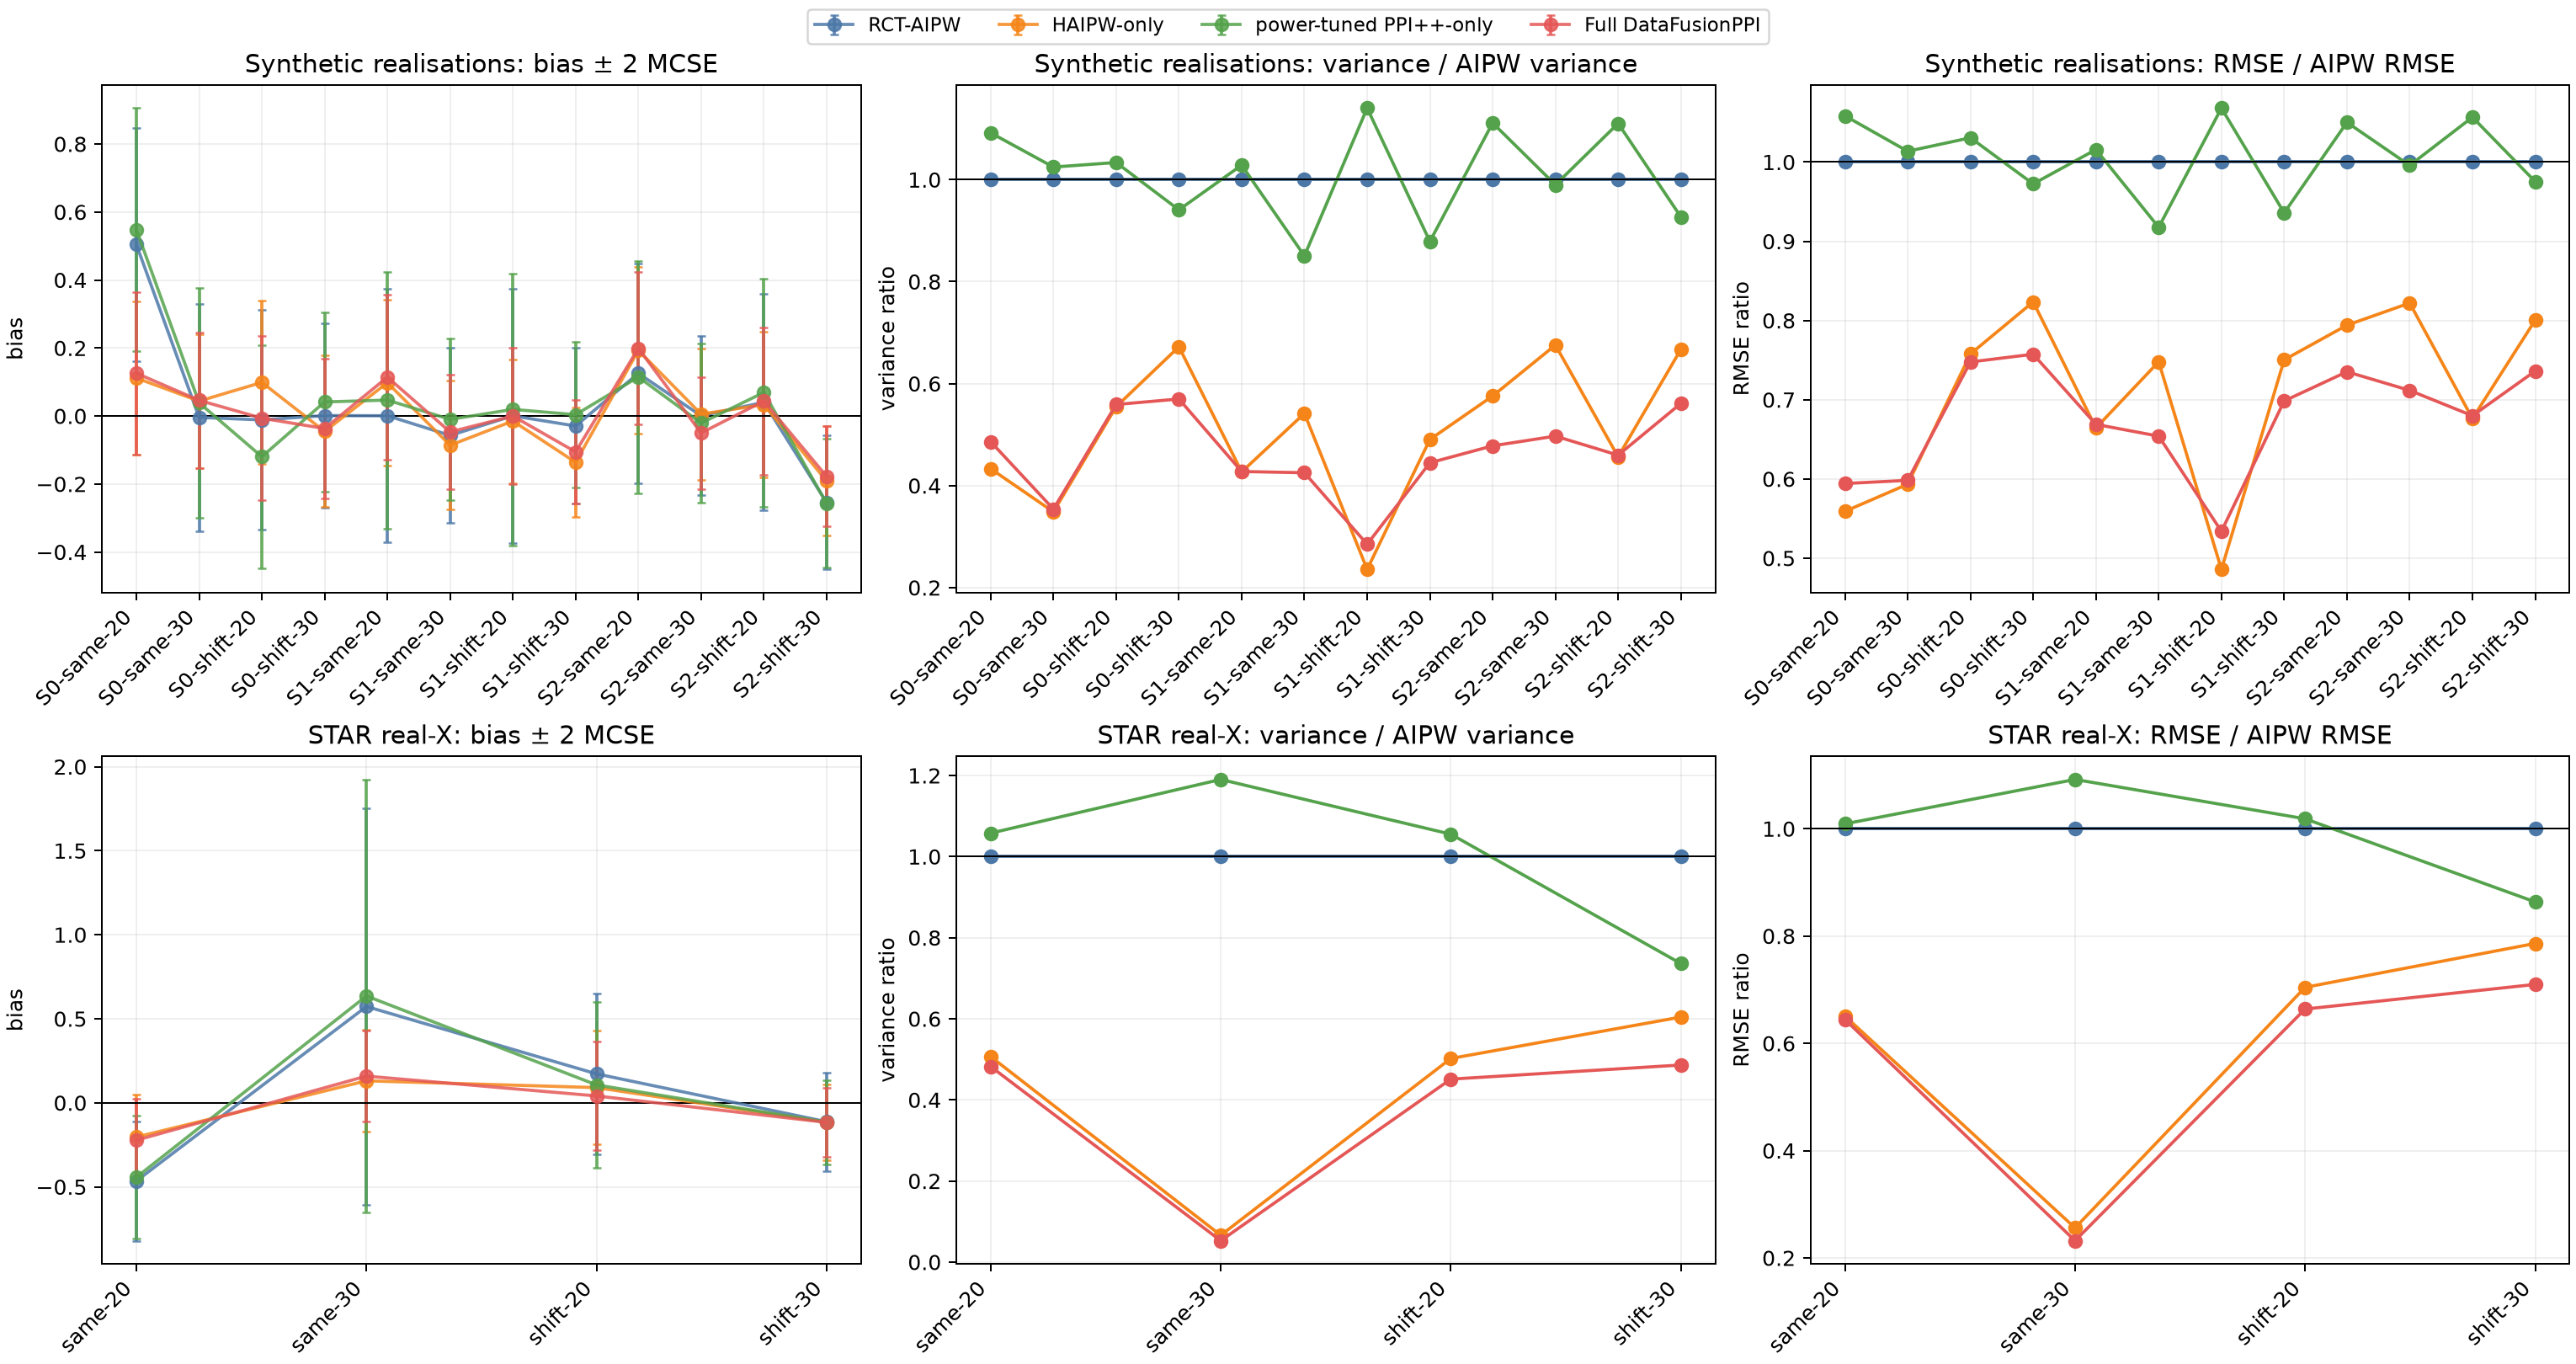
\includegraphics[width=0.98\textwidth]{../materials/total_budget_nested_benchmark.png}
\caption{Fixed-OBS-budget ATE benchmark. The composite artifact reports multiple method and regime panels side by side for $n_R\in\{20,30\}$ and $N_O=5000$.}
\label{fig:fixed-budget}
\end{figure}

\begin{figure}[htbp]
\centering
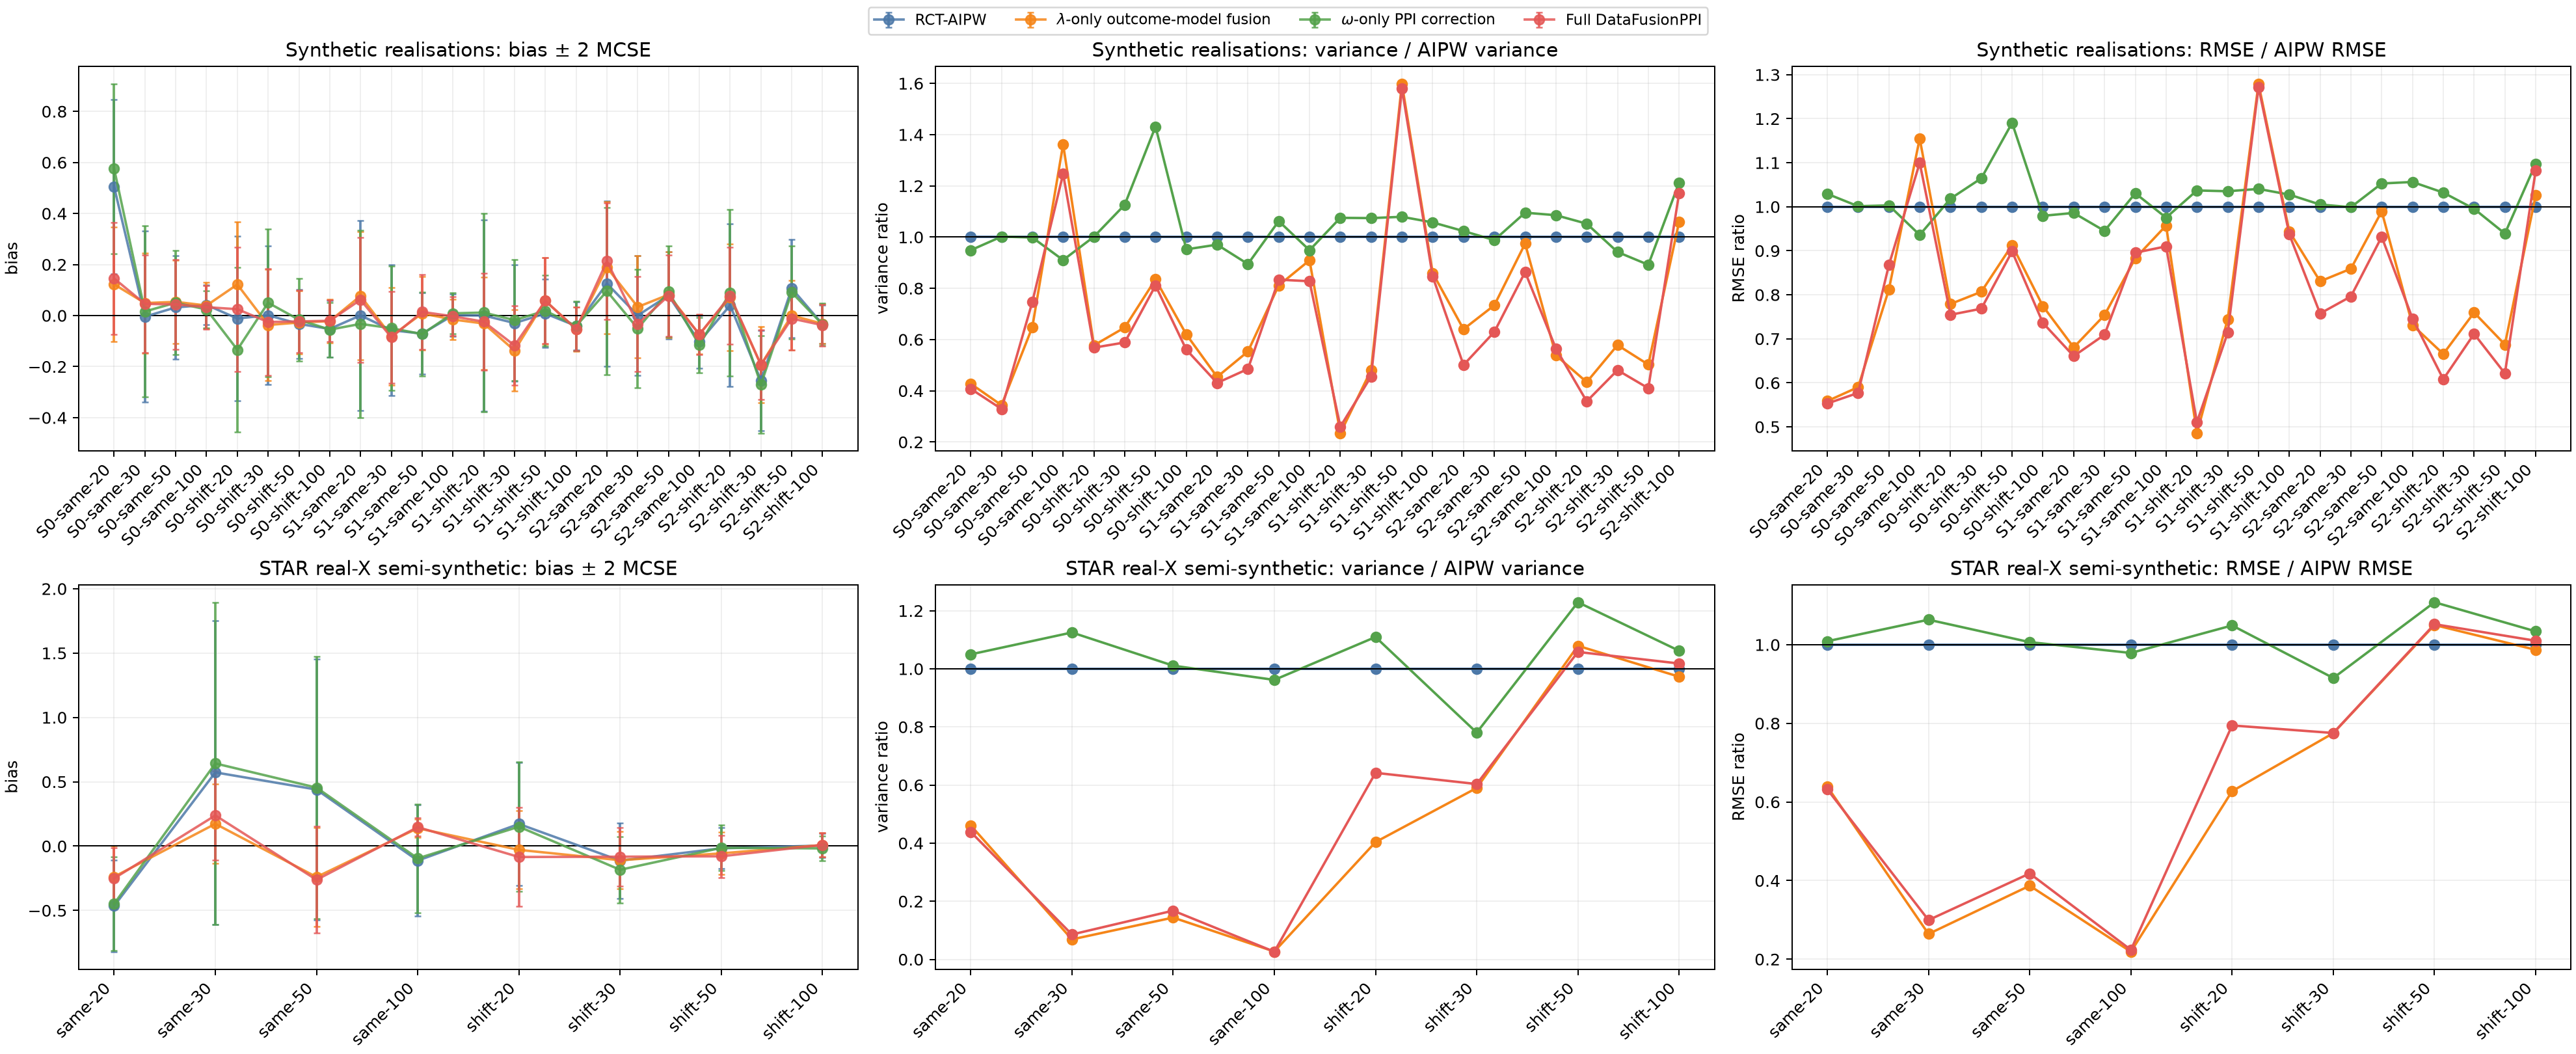
\includegraphics[width=0.98\textwidth]{../materials/proportional_budget_nested_benchmark.png}
\caption{Proportional-budget ATE benchmark. The composite artifact reports multiple method and regime panels side by side for $n_R\in\{20,30,50,100\}$ and $N_O=100n_R$.}
\label{fig:proportional-budget}
\end{figure}

The fixed-OBS-budget benchmark contains 16 design cells: three arbitrary nonlinear SCMs and one STAR real-$X$ construction, each under a common covariate marginal and covariate shift and $n_R\in\{20,30\}$, with $N_O=5000$. The joint estimator has the smallest RMSE in 11 cells, and the $\lambda$-only estimator is best in the remaining five. The joint estimator has lower RMSE than AIPW in all 16 cells, with mean RMSE ratio $0.648$ and mean empirical-variance ratio $0.439$ relative to AIPW. The $\lambda$-only estimator also beats AIPW in all 16 cells, with mean RMSE ratio $0.679$. The $\omega$-only estimator is not best in any cell and has mean RMSE ratio $1.005$.

The proportional-budget benchmark contains 32 cells with $n_R\in\{20,30,50,100\}$ and $N_O=100n_R$. The joint estimator has the smallest RMSE in 18 cells, the $\lambda$-only estimator in 10, the $\omega$-only estimator in one, and AIPW in three. The joint estimator has lower RMSE than AIPW in 27 of 32 cells, with mean RMSE ratio $0.760$ and mean empirical-variance ratio $0.625$. The $\lambda$-only estimator beats AIPW in 28 cells and has mean RMSE ratio $0.769$. The $\omega$-only estimator beats AIPW in 10 cells and has mean RMSE ratio $1.020$. These counts show that joint tuning is often useful but is not uniformly best after coefficient estimation.

The STAR benchmark uses only real kindergarten covariates from Project STAR. Treatment assignments, latent confounding, potential outcomes, and effect heterogeneity are generated synthetically. It is therefore a real-$X$, semi-synthetic benchmark rather than an analysis of STAR's original intervention or outcomes. The planned WHI CT+OS analysis has not been run because participant-level access, a semantic crosswalk, and a survival or censoring extension are still required.

\subsection{Planned CATE evaluation and interpretation}

CATE experiments are planned. The primary design will compare the proved AIPW-pseudo-outcome F-Learner with the prospective R-loss extension using additive cubic B-splines, frozen neural bases, and linear sieves under a common covariate marginal and covariate shift. Each study will compare trial-only, $\lambda$-only, $\omega$-only, and joint tuning using held-out RCT-population CATE risk. Classifier-only, balancing-only, hybrid, and oracle transport weights will be separated. No CATE result is claimed from Figures~\ref{fig:fixed-budget} and \ref{fig:proportional-budget}.

The empirical conclusion is deliberately limited. The two-channel population oracle weakly improves the ATE variance objective when the trial-only coefficient is feasible, but estimated coefficients do not inherit a universal no-harm property. The present 20-repetition studies suggest that the $\lambda$ channel is the more stable source of gain and that joint tuning can add value in some designs. More Monte Carlo repetitions, completed CATE experiments, additional real-$X$ supports, and an authorized real-outcome analysis are required before making a stronger empirical claim.

\subsection{Scope, failure modes, and conclusion}
\label{sec:active-conclusion}

The framework uses observational information through prediction rather than by declaring the observational treatment contrast causal. Trial randomization validates the pseudo-outcome for every fixed outcome regression. A common covariate marginal or an exact density ratio centers the ATE control variate and the prediction-powered CATE loss, which creates separate $\lambda$- and $\omega$-channels while retaining RCT-population targets.

The first boundary is covariate transport. Without weighting under $P_R^X\neq P_O^X$, the ATE correction has drift $\omega\{P_O\widehat{g}-P_R\widehat{g}\}$, and the unweighted CATE loss targets the wrong covariate average. Exact $r=dP_R^X/dP_O^X$ removes both discrepancies. An estimated ratio instead contributes the explicit ATE drift $\omega P_O\{(\widehat r-r)\widehat{g}\}$ and the CATE validation drift in item 3 of Theorem~\ref{thm:cate-finite-validation}. Evaluation-only variance is first-order adequate only under the stated negligible-drift conditions; otherwise ratio-training influence and covariance terms are required.

The second boundary is trial propensity overlap. Proposition~\ref{prop:pseudo-validity-active} uses the known, strictly positive randomized-trial propensity. Extreme inverse-propensity factors can make the required moments unstable even when the conditional-mean identity remains algebraically valid, and an incorrect propensity removes the exact arbitrary-$q$ guarantee.

The third boundary is weak observational prediction. The unrestricted $\omega$-gain depends on how strongly $\widehat{g}(X)$ predicts $\tau(X)$, with attenuation from the finite $n/N$ ratio. The $\lambda$-channel gives little gain when $\Delta=Z_1-Z_0$ is uninformative or nearly degenerate. Population oracles diagnose these limits but do not make their empirical coefficient estimates stable.

The fourth boundary is adaptive reuse. Fitting nuisances, tuning candidates, and evaluating the selected candidate on the same outcomes invalidates the conditioning product law. Present inference therefore uses independent nuisance-fitting, coefficient-tuning, and final-evaluation samples, supplied separately or constructed by splitting. The theory does not cover cross-fitted reuse; that extension requires a separate stability or influence-function analysis.

The fifth boundary is learner restriction and curvature. Target preservation does not make a finite-sample restricted or highly penalized projection accurate. The square-completed representation is a nonnegative mixture only for $0\leq\omega<1$, and positive semidefiniteness at $\omega=1$ must be read from the original quadratic. Coefficients outside $[0,1]$, nonlinear parameterizations, and penalty rescaling require direct analysis of the original objective.

The sixth boundary is tail behavior. ATE variance identities require square-integrable scores; the Wald theorem additionally requires conditional Lindeberg control, a sufficient $(2+\delta)$-moment condition, and a nondegenerate variance limit. Fixed-loss variance tuning imposes fourth-moment-type requirements. Heavy tails can therefore destabilize oracle formulas even when their algebraic denominators are nonzero.

Within these boundaries, the randomized trial fixes the causal target, the OBS outcome model can reduce within-$X$ pseudo-outcome noise through $\lambda$, and the OBS covariate sample can reduce predictable between-$X$ variation through $\omega$. The exact results are conditional identities and population-oracle comparisons. Empirical work must retain the identical trial-only fallback, report selection and denominator instability, and avoid interpreting them as a universal finite-sample no-harm guarantee.

\endgroup

\clearpage
\bibliographystyle{apalike}
\bibliography{reference}

\clearpage
\appendix
\onecolumn

\begingroup
\allowdisplaybreaks
\sloppy
\section{Omitted Preliminaries}
\label{app:omitted-preliminaries}

\subsection{Prediction-powered inference and
\texorpdfstring{PPI\textsuperscript{++}}{PPI++}}
\label{sec:ppi-background}

Let $(X_i,Y_i)$, $i=1,\ldots,n$, be independent and identically distributed labeled observations from a distribution $P$, and let $\widetilde X_j$, $j=1,\ldots,N$, be independent and identically distributed unlabeled covariates from the marginal distribution $P^X$, independently of the labeled sample. Let $f$ be a fixed predictor. For a fixed coefficient $\omega\in\mathbb R$, the PPI\textsuperscript{++} estimator \citep{angelopoulos2024ppipp} of the labeled-population mean is
\begin{align}
	\widehat\mu_{\mathrm{PPI}^{++}}(\omega)
	&\triangleq
	\frac1n\sum_{i=1}^nY_i
	+\omega\left\{
	\frac1N\sum_{j=1}^N f(\widetilde X_j)
	-\frac1n\sum_{i=1}^n f(X_i)
	\right\}.
\end{align}
If $Y$ and $f(X)$ are integrable, then $\widehat\mu_{\mathrm{PPI}^{++}}(\omega)$ is unbiased for $\mathbb E(Y)$ for every fixed $\omega$, because the labeled and unlabeled predictions have the same expectation. The same conclusion holds conditionally when $\omega$ is selected using data independent of the two samples displayed above. PPI\textsuperscript{++} selects $\omega$ to control how strongly this mean-zero prediction difference enters the estimator. When $\operatorname{Cov}\{Y,f(X)\}\neq0$ and $\omega$ is close to its variance-minimizing value, the prediction difference can reduce variance relative to the labeled-only estimator.

\clearpage
\section{Omitted Results}
\label{app:omitted}

\subsection{Convexity of the fusion losses}
\label{app:fusion-convexity}

Step 2 of Algorithm~\ref{alg:cate-fusion-selection} minimizes the losses of Definition~\ref{def:fusion-losses} over $\zeta\in\mathcal Z$. The following expansion shows that this is a convex least-squares problem. It is recorded here because the results of Section~\ref{sec:cate-risk-selection} condition on the fitted function and do not use it.

\begin{proposition}[Convexity of the fusion losses]
\label{prop:fusion-convexity}
Fix $j\in\{\mathrm{DRF},\mathrm{RF}\}$, $\lambda\in[0,1]$, $\omega\in[0,1]$, and $r\geq0$. Expanding the squares in Definition~\ref{def:fusion-losses}, $\widehat L_j(\zeta;\lambda,\omega,r)$ is a quadratic functional of $\zeta$ whose second-order part is
\begin{align}
\text{DRF: }&(1-\omega)\,\mathbb P_R^{\mathrm{tune}}\{\zeta(X)^2\}+\omega\,\mathbb P_O^{\mathrm{tune}}\{r(X)\zeta(X)^2\},
\notag\\
\text{RF: }&(1-\omega)\,\mathbb P_R^{\mathrm{tune}}\{\chi(A,X)\zeta(X)^2\}+\omega\,\mathbb P_O^{\mathrm{tune}}\{r(X)\zeta(X)^2\}.
\label{eq:fusion-curvature}
\end{align}
Both are nonnegative, so $\widehat L_j(\cdot;\lambda,\omega,r)$ is convex on any convex $\mathcal Z$. The expected loss $\mathbb E\{\widehat L_j(\zeta;\lambda,\omega,r)\}$ has the same second-order part with $\mathbb E_R$ and $\mathbb E_O$ in place of $\mathbb P_R^{\mathrm{tune}}$ and $\mathbb P_O^{\mathrm{tune}}$, and is convex as well.
\end{proposition}
Convexity is the condition under which, by Definition~\ref{def:orthogonality}, the minimizers of the expected losses are exactly the zeros of the learning equations in Definition~\ref{def:learning-equations}.

\subsection{Closed-form noise-floor coefficients}
\label{app:noise-floor}

A closed-form choice of $\lambda$ minimizes the noise floors of Proposition~\ref{prop:cate-target} instead of the CATE risk of the fitted learner in Definition~\ref{def:fitted-fusion-learner}. It is recorded here because the validation route of Section~\ref{sec:cate-risk-selection} targets the fitted risk directly and also chooses $\omega$.

\begin{proposition}[Noise-floor coefficients]
\label{prop:cate-noise-floor-lambda}
Suppose Assumptions~\ref{ass:trial} and~\ref{ass:honest-separation} hold and the displayed moments are finite. Recall $Z_0$, $Z_1$, and $\Delta=Z_1-Z_0$ from Section~\ref{sec:rct-obs-setting}, so that $Z_\lambda=Z_0+\lambda\Delta$, and write $d_m\triangleq m_O-m_R$, so that $m_\lambda=m_R+\lambda d_m$. Let $\operatorname{Proj}_{[0,1]}(u)\triangleq\min\{1,\max(0,u)\}$. If $\mathbb E_R(\Delta^2)>0$, then
\begin{align}
\operatorname*{arg\,min}_{\lambda\in[0,1]}Q_{\mathrm{DR}}(\lambda)
&=\operatorname{Proj}_{[0,1]}\left\{-\frac{\mathbb E_R(Z_0\Delta)}{\mathbb E_R(\Delta^2)}\right\},
\label{eq:cate-dr-noise-lambda}
\end{align}
and if $\mathbb E_R[d_m(X)^2/\{e(X)(1-e(X))\}]>0$, then
\begin{align}
\operatorname*{arg\,min}_{\lambda\in[0,1]}Q_R(\lambda)
&=\operatorname{Proj}_{[0,1]}\left[
\frac{\mathbb E_R[\{Y-m_R(X)\}d_m(X)/\{e(X)(1-e(X))\}]}
{\mathbb E_R[d_m(X)^2/\{e(X)(1-e(X))\}]}\right].
\label{eq:cate-r-noise-lambda}
\end{align}
If a denominator is zero, the corresponding noise floor is constant in $\lambda$. Both minimizers can be estimated by replacing the moments with tuning-sample averages.
\end{proposition}

\clearpage
\section{Simulation Details}
\label{app:simulations}

All completed simulation artifacts were generated with base seed $190602$.  The
primary nested benchmarks use $20$ outer Monte Carlo repetitions per design
cell and compare four estimators: RCT-only AIPW, $\lambda$-only outcome-model
fusion, $\omega$-only PPI correction, and joint $(\lambda,\omega)$ fusion.
The implementation retains the historical internal codes
\texttt{haipw\_only} and \texttt{ppi\_power\_tuned\_only} for the second and
third estimators, respectively.  These codes are not the user-facing method
names, and the first does not refer to the separate HAIPW paper.

The arbitrary simulation family uses three nonlinear structural causal models.
In every model, a domain indicator $S$ distinguishes the observational sample
($S=0$) from the randomized sample ($S=1$); covariates depend on latent
variables, observational treatment depends on both measured covariates and an
unmeasured confounder, trial treatment follows the known randomized propensity,
and outcomes may depend nonlinearly on covariates, treatment, and the latent
confounder.  The common-marginal regime uses $P_R^X=P_O^X$.  The shifted
regime changes the covariate distribution while preserving overlap and estimates
the density ratio from a domain classifier.  The same estimators and evaluation
logic are used in both regimes.

The fixed-OBS-budget experiment has $16$ cells: four benchmark families, two
covariate regimes, and $n_R\in\{20,30\}$, with $N_O=5000$.  The proportional
experiment has $32$ cells: four benchmark families, two regimes, and
$n_R\in\{20,30,50,100\}$, with the exact mapping
$N_O=100n_R\in\{2000,3000,5000,10000\}$.  Coefficients are estimated by the
nested honest procedure; no oracle coefficient or oracle density ratio is used
in the reported method comparison.  The replication-level CSV files, summaries,
and composite plots in \texttt{materials/} are the canonical numerical artifacts.

The fourth benchmark family reuses the empirical covariate support from the
Tennessee Student/Teacher Achievement Ratio (STAR) experiment.  Treatment,
latent confounding, outcomes, and treatment-effect heterogeneity are generated by
the benchmark code.  Consequently this is a real-$X$, semi-synthetic design,
not an evaluation of the original STAR outcomes or intervention effect.

Figure~\ref{fig:pilot} records the earlier two-method pilot.  It is retained for
provenance but is not the basis for the four-method conclusions in
Section~\ref{sec:experiments}.

\begin{figure}[htbp]
\centering
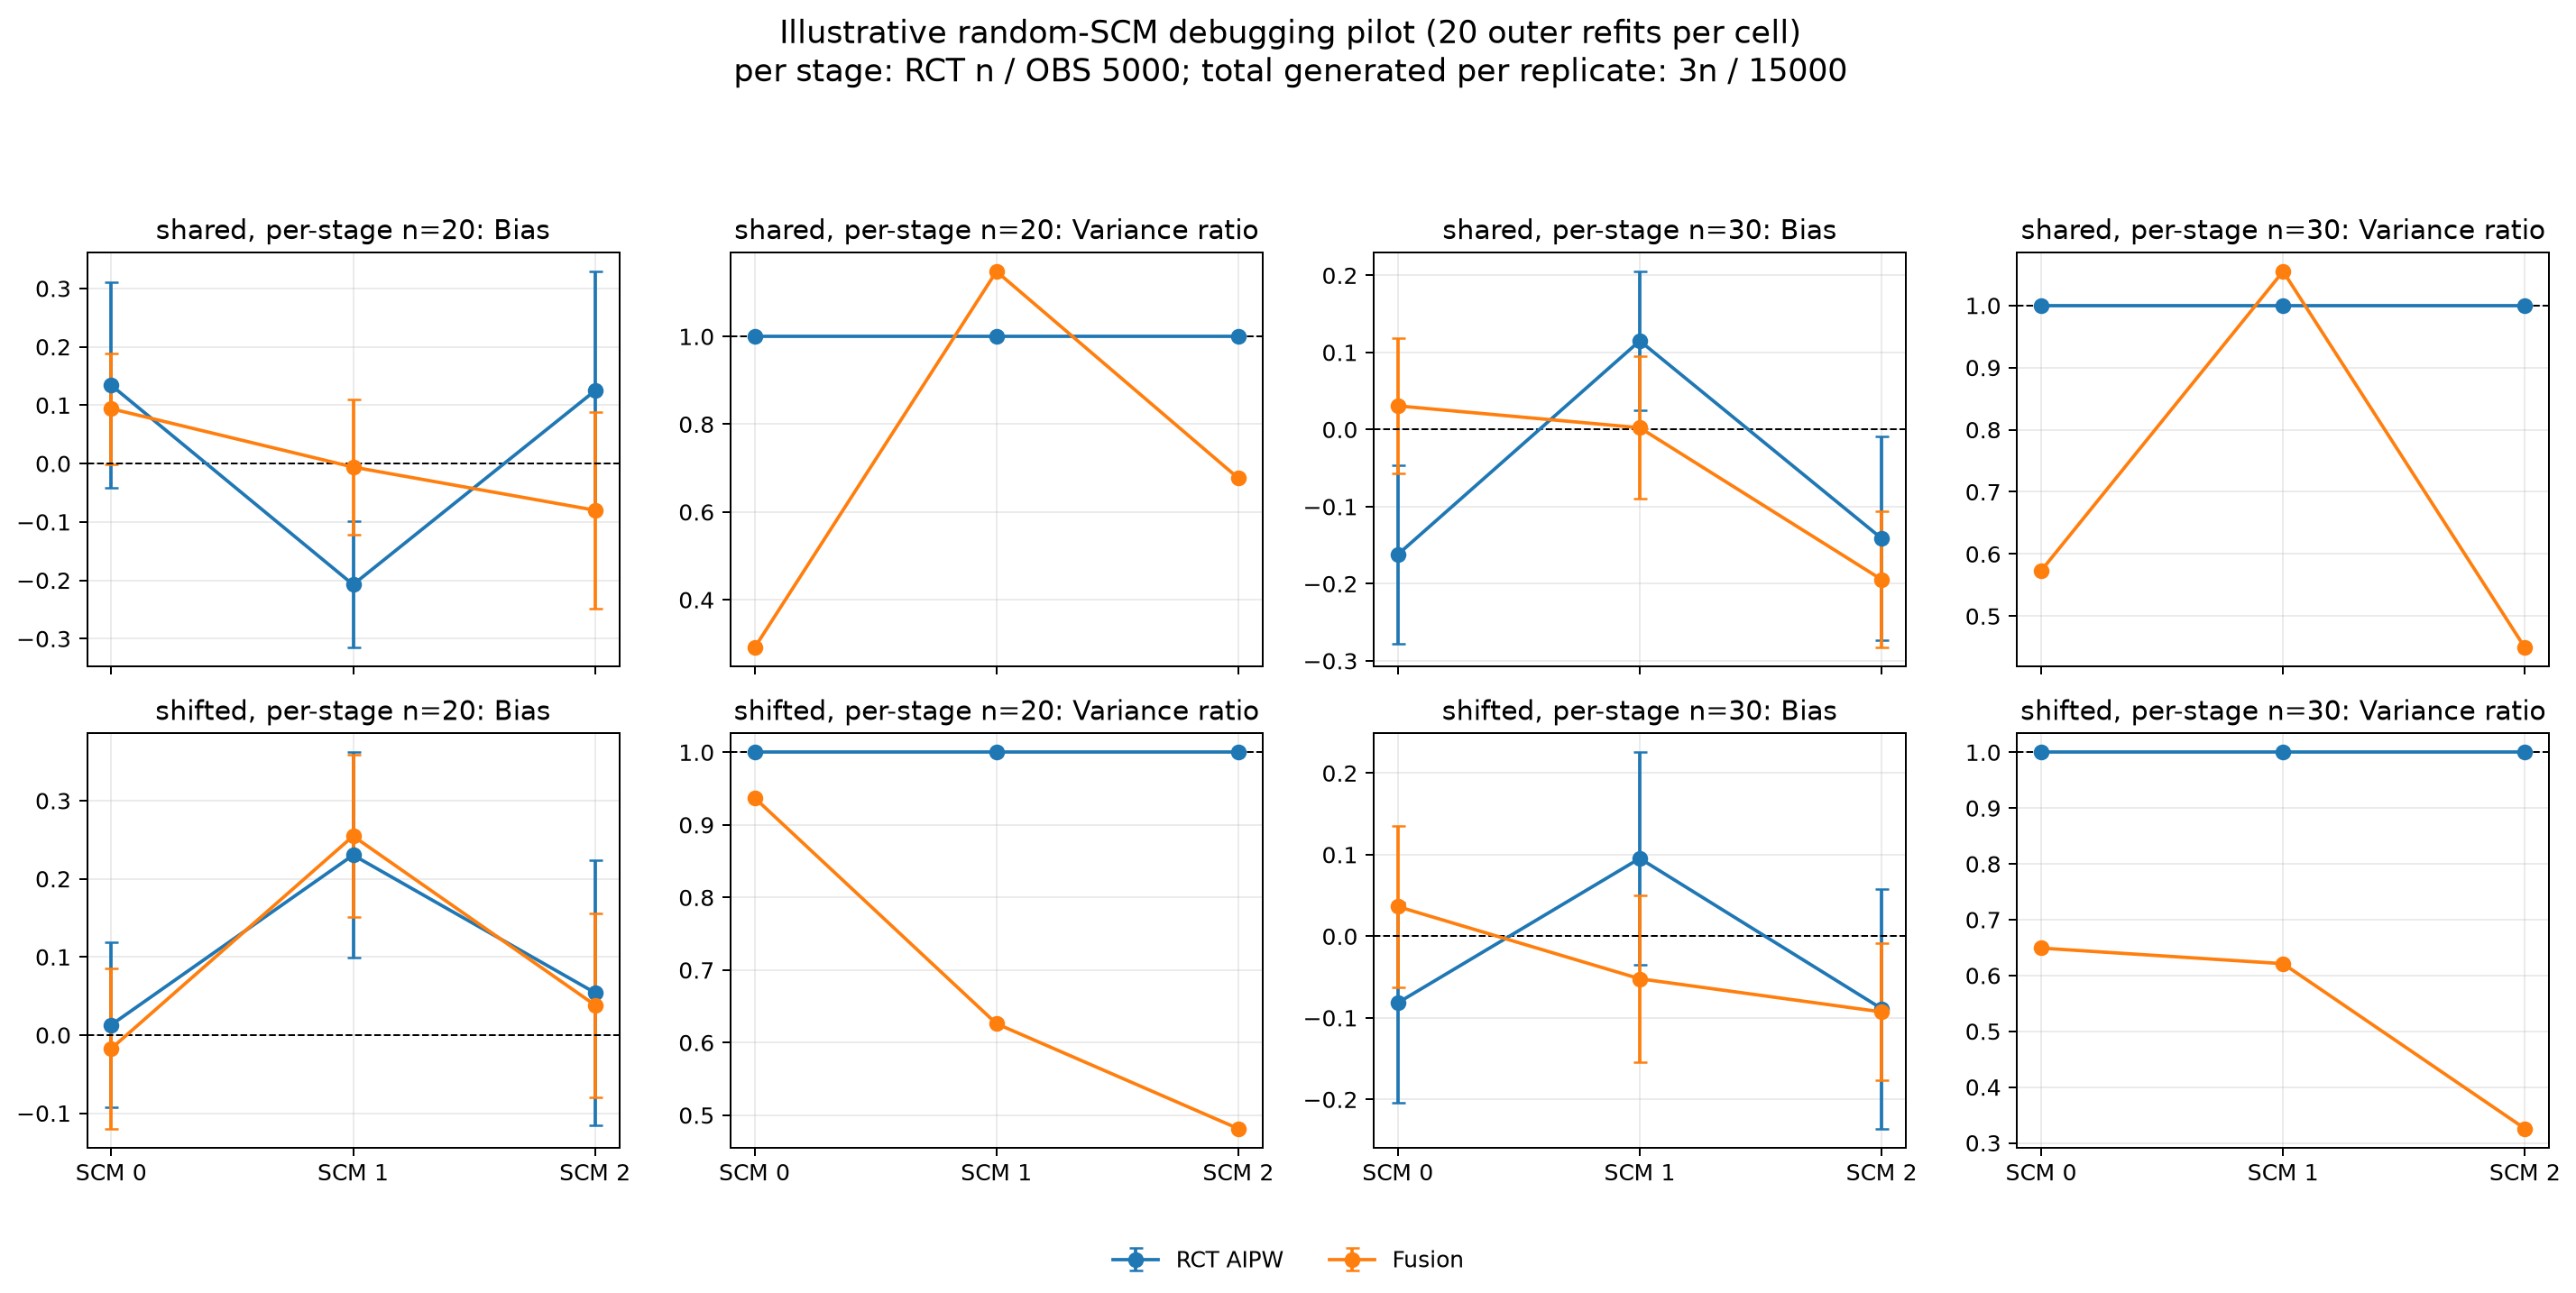
\includegraphics[width=0.98\textwidth]{../materials/ssem_ate_pilot.png}
\caption{Earlier SSEM ATE pilot.  This artifact predates the nested four-method
comparison and should be interpreted only as a design and implementation check.}
\label{fig:pilot}
\end{figure}

No participant-level WHI CT+OS analysis is included.  Such an analysis requires
authorized data access, a verified trial--observational semantic crosswalk, a
prespecified estimand, and methods appropriate for censoring if the selected
outcome is time-to-event.  No completed CATE experiment or real-outcome result is
represented by the present artifacts.

\clearpage
\section{Proof Details}
\label{app:proofs}

\subsection{Conditional validity of the trial pseudo-outcome}

Fix \(q=(q_0,q_1)\) and condition on \(X\).  Under trial randomization and
consistency,
\begin{align}
\mathbb E_R\left[\frac{A}{e(X)}\{Y-q_1(X)\}\mid X\right]
&=\mathbb E_R\{Y(1)-q_1(X)\mid X\},
\\
\mathbb E_R\left[\frac{1-A}{1-e(X)}\{Y-q_0(X)\}\mid X\right]
&=\mathbb E_R\{Y(0)-q_0(X)\mid X\}.
\end{align}
Substituting these two equalities into the definition of \(\varphi\) cancels the
two fitted regressions and yields
\(\mathbb E_R\{\varphi(V;q)\mid X\}=\tau(X)\).  Applying the identity to
\(q=\widehat\mu_R\), \(q=\widehat\mu_O\), and their affine blend gives
\begin{align}
\mathbb E_R(Z_\lambda\mid X)&=\tau(X),
&
\mathbb E_R(\Delta\mid X)&=0.
\end{align}
These statements are conditional on the pre-evaluation sigma-field so that the
fitted functions are fixed.

\subsection{Proof of Theorem~\ref{thm:ate-variance}}

Using \(\mathbb E_R(Z_\lambda)=\theta\) and exact transport,
\begin{align}
\mathbb E_O\{r(X)g(X)\}=\mathbb E_R\{g(X)\},
\end{align}
the conditional mean of Equation~\eqref{eq:ate-estimator} is \(\theta\).  Rewrite
the centered estimator as
\begin{align}
\widehat\theta_r(\lambda,\omega)-\theta
&=
(\mathbb P_{R,n}-P_R)\{Z_\lambda-\omega g\}
+(\mathbb P_{O,N}-P_O)\{\omega rg\}.
\end{align}
The two summands are independent conditional on \(\mathcal F\).  The variance of
an empirical mean of \(m\) independent observations is the population variance
divided by \(m\), which proves Equation~\eqref{eq:ate-variance}.  Unbiased sample
variances on the two independent evaluation blocks therefore give the displayed
fixed-selected-coefficient variance estimator in Section~\ref{sec:ate}.  Coverage
of its Wald interval additionally uses the stated conditional Lindeberg and
moment assumptions; variance unbiasedness alone is not a central limit theorem.

If an estimated ratio \(\widehat r\) replaces \(r\), the conditional mean changes
by exactly
\begin{align}
\omega P_O\{(\widehat r-r)g\}.
\end{align}
Thus honest evaluation does not restore exact unbiasedness.  Negligibility of
both the root-\(n\) drift and the OBS empirical remainder is required before the
fixed-ratio evaluation variance can be used as a first-order variance formula.

\subsection{Proof of Theorem~\ref{thm:joint-oracle}}

Expand the first variance in Equation~\eqref{eq:ate-variance} using
\(Z_\lambda=Z_0+\lambda\Delta\).  After collecting terms and multiplying by
\(n\), the coefficient-dependent part is
\begin{align}
2C\lambda-2D\omega+A\lambda^2-2E\lambda\omega+B\omega^2,
\end{align}
which is \(2\ell^\top\beta+\beta^\top\mathbf H\beta\).  The representation
\begin{align}
\begin{pmatrix}u&v\end{pmatrix}\mathbf H\begin{pmatrix}u\\v\end{pmatrix}
&=\operatorname{Var}_R(u\Delta-vg)
+\frac nN v^2\operatorname{Var}_O(rg)
\end{align}
proves positive semidefiniteness.  If \(AB-E^2>0\), the first-order condition
\(\mathbf H\beta=-\ell\) has the unique solution
\begin{align}
\lambda^\star&=\frac{ED-BC}{AB-E^2},
&
\omega^\star&=\frac{AD-EC}{AB-E^2}.
\end{align}
When \(\mathbf H\) is singular, nonnegativity of the variance quadratic implies
\(\ell\in\operatorname{Range}(\mathbf H)\); otherwise a null-space direction
would make the expression arbitrarily negative.  The complete minimizer set is
therefore \(-\mathbf H^+\ell+\operatorname{Null}(\mathbf H)\).  Continuity of the
quadratic proves attainment on every prespecified compact feasible set.

Finally, because \(g\) is \(X\)-measurable,
\begin{align}
E
&=\mathbb E_R[\{g(X)-P_Rg\}\mathbb E_R(\Delta\mid X)]=0,
\\
D
&=\operatorname{Cov}_R\{\mathbb E_R(Z_0\mid X),g(X)\}
=\operatorname{Cov}_R\{\tau(X),g(X)\}.
\end{align}
Substitution yields Equation~\eqref{eq:axis-oracle}.  Since the population
objective is minimized over a set containing \((0,0)\), its oracle value cannot
exceed the trial-only value.  This comparison concerns the population objective,
not coefficients estimated from a finite tuning sample.

\subsection{Proof of Corollary~\ref{cor:joint-oracle-variance}}

Write the conditional variance as
\begin{align*}
V(\beta)
&=
V_0+
\frac1n
\{2\ell^\top\beta+\beta^\top\mathbf H\beta\},
&
V_0
&=
\frac1n\operatorname{Var}_R(Z_0).
\end{align*}
When \(AB-E^2>0\), the matrix \(\mathbf H\) is positive definite and the unique minimizer is \(\beta^\star=-\mathbf H^{-1}\ell\). Substitution gives
\begin{align*}
V(\beta^\star)
&=
V_0-
\frac1n\ell^\top\mathbf H^{-1}\ell.
\end{align*}
For \(\mathbf H=\left(\begin{smallmatrix}A&-E\\-E&B\end{smallmatrix}\right)\),
\begin{align*}
\mathbf H^{-1}
&=
\frac1{AB-E^2}
\begin{pmatrix}B&E\\E&A\end{pmatrix},
\\
\ell^\top\mathbf H^{-1}\ell
&=
\frac{BC^2-2ECD+AD^2}{AB-E^2}.
\end{align*}
Positive definiteness makes this quadratic form nonnegative and makes it zero exactly when \(\ell=0\). Setting \(E=0\) yields \(C^2/A+D^2/B\).

If \(\mathbf H\) is singular, boundedness below of the variance objective implies \(\ell\in\operatorname{Range}(\mathbf H)\). Evaluating at the minimum-norm solution \(-\mathbf H^+\ell\) gives
\begin{align*}
V_{\min}
&=
V_0-
\frac1n\ell^\top\mathbf H^+\ell.
\end{align*}
The pseudoinverse is positive definite on \(\operatorname{Range}(\mathbf H)\), so the reduction is strictly positive exactly when \(\ell\neq0\). Finally, continuity gives attainment on every nonempty compact feasible set \(\mathcal C\). If \(0\in\mathcal C\), the constrained minimum is at most \(V(0)=V_0\), and it is strictly smaller exactly when some feasible \(\beta\) makes \(2\ell^\top\beta+\beta^\top\mathbf H\beta<0\).

\subsection{Prediction-powered CATE risk identity}

Fix \(t\) and condition on \(X\).  Since
\(\mathbb E_R(Z_\lambda-\tau(X)\mid X)=0\),
\begin{align}
\mathbb E_R\{Z_\lambda-t(X)\}^2
&=
\mathbb E_R\{Z_\lambda-\tau(X)\}^2
+\mathbb E_R\{t(X)-\tau(X)\}^2.
\end{align}
Exact transport also gives
\begin{align}
\mathbb E_O\{r(X)(g(X)-t(X))^2\}
&=\mathbb E_R\{(g(X)-t(X))^2\}.
\end{align}
The correction in Equation~\eqref{eq:dr-fusion-loss} therefore has mean zero,
which proves Equation~\eqref{eq:cate-target}.  In particular, population expected
loss is flat in \(\omega\).  The part depending on \(\lambda\) is
\begin{align}
Q(\lambda)
&=Q(0)+2C\lambda+A\lambda^2,
\end{align}
so when \(A>0\) its minimizer is \(-C/A\), the same integrated-noise oracle as
in the population-orthogonal ATE problem.  If \(A=0\), then \(\Delta=0\) almost
surely by conditional mean zero, and \(Q\) is flat in \(\lambda\).

For a fixed \(t\) and \(\lambda\), the empirical loss is the sum of independent
empirical means of \(U_{t,\lambda}-\omega G_t\) under the trial and
\(\omega rG_t\) under the observational law.  Expanding its variance as a
quadratic in \(\omega\) and differentiating gives
Equation~\eqref{eq:loss-variance-omega}.  Because \(t\) is fixed in this
calculation, the formula does not identify the coefficient minimizing the risk
of a learner chosen after seeing the same loss.

For the linear sieve, expand Equation~\eqref{eq:dr-fusion-loss} in \(\beta\), add
\(\rho\beta^\top P\beta\), and set the gradient to zero.  The resulting normal
equation is
\begin{align}
\{(1-\omega)H_R+\omega H_{O,r}+\rho P\}\beta
&=h_\lambda+\omega d_g,
\end{align}
which proves Equation~\eqref{eq:linear-sieve} whenever the matrix is invertible.

\subsection{Loss-targeted balance and approximate drift}

Suppose a nonnegative out-of-sample-evaluable weight \(w\) satisfies
\begin{align}
P_O\{w(g-t)^2\}=P_R\{(g-t)^2\}
\quad\text{for every }t\in\mathcal T.
\end{align}
Replacing \(r\) by \(w\) then leaves the population correction exactly zero for
every candidate, so the target identity remains valid.  If
\(t_\beta=b^\top\beta\), expanding
\begin{align}
(g-b^\top\beta)^2
&=g^2-2\beta^\top bg+\beta^\top bb^\top\beta
\end{align}
shows that balancing \(bg\) and \(bb^\top\) preserves the minimizer.  Balancing
\(g^2\) is needed only to preserve the absolute loss value.

For approximate weights, the difference between the weighted and target
population losses is bounded uniformly over \(\mathcal T\) by
\(|\omega|\Delta_\mathcal T(w)\).  Let \(t_w\) minimize the weighted population
loss and \(t_0\) minimize the target loss.  Applying the uniform bound at both
minimizers gives
\begin{align}
L_0(t_w)
&\leq L_w(t_w)+|\omega|\Delta_\mathcal T(w)
\\
&\leq L_w(t_0)+|\omega|\Delta_\mathcal T(w)
\\
&\leq L_0(t_0)+2|\omega|\Delta_\mathcal T(w),
\end{align}
which is the claimed excess-risk bound.  If the same finite sample is used both
to impose exact sieve balance and to fit \(\beta\), the balanced linear and
quadratic coefficient terms cancel from the empirical correction (and the
constant cancels as well if \(g^2\) is balanced).  This algebra explains why
weight learning and candidate fitting require honest separation or a separate
outer-fold argument.

\endgroup

\end{document}
